\documentclass[a4paper,twoside]{article}
\usepackage[utf8]{inputenc}

\usepackage{bcprules}
\usepackage{prooftree}
\usepackage{amsthm}
\usepackage{amsmath}
\usepackage{amssymb}
\usepackage{mathpartir}
\usepackage{enumitem}

\newtheorem{thm}{Theorem}[section]
% \newtheorem{corollary}{Corollary}[thm]
% \newtheorem{lemma}[thm]{Lemma}
\newtheorem{defn}{Definition}[section]
\newtheorem*{thmun}{Theorem}
\newtheorem*{lemmaun}{Lemma}

%%% Syntax

%%% Operational model
\newcommand{\Req}[3]{\text{Req}_s(#1, #2, #3)}
\newcommand{\Res}[3]{\text{Res}_s(#1, #2, #3)}
\newcommand{\ReqF}[2]{\text{Req}_{\iota}(#1, #2)}
\newcommand{\ReqE}[3]{\text{Req}_f(#1, #2, #3)}
\newcommand{\Per}[3]{\text{Persist}(#1, #2, #3)}

%%% Calculus abbreviations
\newcommand{\None}{\text{None}}
\newcommand{\Some}[1]{\text{Some}(#1)}

\newcommand{\Val}[1]{\text{Val}(#1)}
\newcommand{\Fwd}[1]{\text{Fwd}(#1)}

%% Util
\newcommand{\consume}[3]{\text{consume}(#1, #2, #3)}

%% Misc
\newcommand{\note}[1]{{\bf $\clubsuit$ #1 $\spadesuit$}}

\renewcommand{\text}[1]{\textrm{#1}}

% Member sequences
\newcommand{\seq}[1]{\overline{#1}}

% arrays
\newcommand{\ba}{\begin{array}}
\newcommand{\ea}{\end{array}}
\newcommand{\bda}{\[\ba}
\newcommand{\eda}{\ea\]}
\newcommand{\ei}{\end{array}}
\newcommand{\bcases}{\left\{\begin{array}{ll}}
\newcommand{\ecases}{\end{array}\right.}

% spacing
\newcommand{\gap}{\quad\quad}
\newcommand{\biggap}{\quad\quad\quad}
\newcommand{\nextline}{\\ \\}
\newcommand{\htabwidth}{0.5cm}
\newcommand{\tabwidth}{1cm}
\newcommand{\htab}{\hspace{\htabwidth}}
\newcommand{\tab}{\hspace{\tabwidth}}
\newcommand{\linesep}{\ \hrulefill \ \smallskip}

\newtheorem{theorem}{Theorem}[section]
\newtheorem{lemma}[theorem]{Lemma}
\newtheorem{proposition}[theorem]{Proposition}
\newtheorem{corollary}[theorem]{Corollary}

\newenvironment{definition}[1][Definition]{\begin{trivlist}
\item[\hskip \labelsep {\bfseries #1}]}{\end{trivlist}}
\newenvironment{example}[1][Example]{\begin{trivlist}
\item[\hskip \labelsep {\bfseries #1}]}{\end{trivlist}}
\newenvironment{remark}[1][Remark]{\begin{trivlist}
\item[\hskip \labelsep {\bfseries #1}]}{\end{trivlist}}

\title{The Function Passing Model: Types, Proofs, and Semantics}
\author{Philipp Haller, Normen M\"{u}ller, Heather Miller}
\date{May 2016}

\begin{document}
\maketitle

\section{Overview}
% This section presents a formalization of our type system.

%%%%%%%%%%%%%%%%%%%%%%%%%%%%%%%%%%%%%%%%%%%%%%%%%%%%%%%%%%%%%%
%
% Core language abstract syntax.
%
%%%%%%%%%%%%%%%%%%%%%%%%%%%%%%%%%%%%%%%%%%%%%%%%%%%%%%%%%%%%%%

\begin{figure}[ht!]
\centering

$\ba[t]{l@{\hspace{2mm}}l}
t ::=                                                                  & \mbox{{\it{terms:}}} \\
\gap \:\:\:\:  x                                                       & \mbox{variable} \\
\gap ~|~  (x: T) \Rightarrow t                                         & \mbox{abstraction} \\
\gap ~|~  t~t                                                          & \mbox{application} \\
\gap ~|~  \{ \seq{l = t} \}                                            & \mbox{record construction} \\
\gap ~|~  t.l                                                          & \mbox{selection} \\
\gap ~|~  \texttt{spore}~\{~\seq{x : T = t}~; (x: T) \Rightarrow t~\}  & \mbox{spore} \\
\gap ~|~  \texttt{spawn}(t)                                            & \mbox{spawn host} \\
\gap ~|~  \texttt{populate}(t, t)                                      & \mbox{populate silo} \\
\gap ~|~  \texttt{map}(t, t)                                           & \mbox{map} \\
\gap ~|~  \texttt{flatMap}(t, t)                                       & \mbox{flatMap} \\
\gap ~|~  \texttt{persist}(t)                                          & \mbox{persist} \\
\gap ~|~  \texttt{send}(t)                                             & \mbox{send} \\           % send  :: Ref a -> Fut a
\gap ~|~  \texttt{await}(t)                                            & \mbox{await future} \\   % await :: Fut a -> a
\gap ~|~  \iota                                                        & \mbox{location} \\
\gap ~|~  r                                                            & \mbox{silo reference} \\
                                                                       & \\
v ::=                                                                  & \mbox{{\it{values:}}} \\
\gap \:\:\:\: (x: T) \Rightarrow t                                     & \mbox{abstraction value} \\
\gap ~|~  \{ \seq{l = v} \}                                            & \mbox{record value} \\
\gap ~|~  p                                                            & \mbox{spore value} \\
\gap ~|~  \iota                                                        & \mbox{location} \\
\gap ~|~  r                                                            & \mbox{silo reference} \\
                                                                       & \\
p ::= \texttt{spore}~\{~\seq{x : T = v}~; (x: T) \Rightarrow t~\}      & \\
& \\
r ::=                                                  & \mbox{{\it{silo reference values:}}} \\
\gap \:\:\:\: \text{Mat}(\omega)                       & \mbox{materialized}                  \\
\gap ~|~  \text{Mapped}(\omega, r, p)                  & \mbox{lineage with \texttt{map}}     \\
\gap ~|~  \text{FMapped}(\omega, r, p)                 & \mbox{lineage with \texttt{flatMap}} \\
\gap ~|~  \text{Persist}(\omega, r, v)                 & \mbox{lineage with \texttt{persist}} \\
                                                       & \\
\omega  ::= (h,i) \quad \text{where}~i \in \mathbb{N}  & \mbox{decentralized identifier}      \\
& \\
T ::=                                                                  & \mbox{{\it{types:}}} \\
\gap \:\:\:\: T \Rightarrow T                                          & \mbox{abstraction type} \\
\gap ~|~  \{ \seq{l : T} \}                                            & \mbox{record type} \\
\gap ~|~  T \Rightarrow T~\{~\texttt{type}~\mathcal{C} = \seq{T}~\}    & \mbox{spore type} \\
\gap ~|~  \texttt{Host}                                                & \mbox{host type} \\
\gap ~|~  \texttt{SiloRef}[T]                                          & \mbox{silo reference type} \\
\gap ~|~  \texttt{Future}[T]                                           & \mbox{future type}
\ea$
\caption{Abstract syntax of core language.}\label{fig:syntax}
\end{figure}

We formalize our programming model in the context of a typed lambda
calculus with records. Figure~\ref{fig:syntax} shows the abstract
syntax of our core language. Besides standard terms, the language
includes terms related to (a) spores, (b) silos, and (c) futures. The
\verb|spore| term creates a new spore. It contains a list of variable
definitions, the spore header, and a closure which may only refer to
its parameter and variables in the spore header. The \verb|spawn| term
creates a new host capable of hosting silos. The \verb|populate| term
initializes a new silo on a given host with a given data value.  The
\verb|map|, \verb|flatMap|, and \verb|persist| terms create lineages
of silo transformations represented as silo references.  The
\verb|send| term forces the materialization of the silo corresponding
to its argument silo reference; \verb|send| returns a future which is
asynchronously completed with the silo's value. The \verb|await| term
waits for the completion of its argument future and returns the
future's value.  Locations $\iota$ are used to refer to futures and
hosts, both of which can be created dynamically using the above terms.

Values in our language are as expected: besides abstractions and
record values they include spore values, locations, and silo
references. Locations and silo references are not part of the
``surface syntax'' of our language; they are only introduced by
evaluation (see Section~\ref{sec:opsem}). Silo reference values are
values of a simple datatype with constructors {\em Mat, Mapped,
  FMapped}, and {\em Persist}. The constructors include all
information required for {\em materializing} a silo with the result of
applying the described transformations. Therefore, a silo reference
value is also called the {\em lineage} of its corresponding silo. We
defer a detailed explanation of the transformations described by a
lineage to the following Section~\ref{sec:opsem}.

In addition to standard function and record types, the language has
types for spores, hosts, silo references, and futures. A spore type $T
\Rightarrow T'~\{~\texttt{type}~\mathcal{C} = \seq{T}~\}$ includes the
types $\seq{T}$ of the variables declared in the header of the spore.

\subsection{Operational Semantics}\label{sec:opsem}

In the following we present a small-step operational semantics of the
introduced core language. The semantics is clearly stratified into a
deterministic layer and a non-deterministic (concurrent)
layer. Importantly, this means our programming model can benefit from
existing reasoning techniques for sequential programs. Program
transformations that are correct for sequential programs are also
correct for distributed programs. Our programming model shares this
property with some existing approaches~\cite{ConcurrentHaskell}.

\begin{figure}
\centering
 $\ba[t]{l@{\hspace{2mm}}l}
E ::=                                                                                                     & \mbox{\it{evaluation contexts:}} \\
\gap \:\:\:\: [~]                                                                                         & \mbox{hole} \\
\gap ~|~  E~t                                                                                             & \mbox{application (fun)} \\
\gap ~|~  v~E                                                                                             & \mbox{application (arg)} \\
\gap ~|~  \{ \seq{l = v} ; l_i = E ; \seq{l' = t} \}                                                      & \mbox{record} \\
\gap ~|~  E.l                                                                                             & \mbox{selection} \\
\gap ~|~  \texttt{spore}~\{~\seq{x : T = v} ; x_i : T_i = E ; \seq{x' : T = t} ; (x: T) \Rightarrow t~\}  & \mbox{spore} \\
\gap ~|~  \texttt{spawn}(E)                                                                               & \mbox{spawn} \\
\gap ~|~  \texttt{populate}(E, t)                                                                         & \mbox{populate (host)} \\
\gap ~|~  \texttt{populate}(v, E)                                                                         & \mbox{populate (spore)} \\
\gap ~|~  \texttt{map}(E, t)                                                                              & \mbox{map (ref)} \\
\gap ~|~  \texttt{map}(v, E)                                                                              & \mbox{map (fun)} \\
\gap ~|~  \texttt{flatMap}(E, t)                                                                          & \mbox{flatMap (ref)} \\
\gap ~|~  \texttt{flatMap}(v, E)                                                                          & \mbox{flatMap (fun)} \\
\gap ~|~  \texttt{persist}(E)                                                                             & \mbox{persist} \\
\gap ~|~  \texttt{send}(E)                                                                                & \mbox{send} \\
\gap ~|~  \texttt{await}(E)                                                                               & \mbox{await} \\
\ea$
\caption{Evaluation context.}\label{fig:eval-ctx}
\end{figure}

The semantics is based on three reduction relations for (a) sequential
reduction of terms, (b) deterministic reduction of hosts, and (c)
non-deterministic reduction of sets of hosts.  The reduction relations
use the definition of evaluation contexts shown in
Figure~\ref{fig:eval-ctx}. Evaluation contexts capture the notion of
the ``next subterm to be evaluated.'' Following a standard
approach~\cite{TAPL}, we write $E[t]$ for the term obtained by
replacing the hole in evaluation context $E$ with term $t$.

%%%%%%%%%%%%%%%%%%%%%%%%%%%%%%%%%%%%%%%%%%%%%%%%%%%%%%%%%%%%%%
%
% Lambda reduction.
%
%%%%%%%%%%%%%%%%%%%%%%%%%%%%%%%%%%%%%%%%%%%%%%%%%%%%%%%%%%%%%%

\begin{figure}
\centering
\begin{mathpar}
\inferrule[\textsc{R-AppAbs}] {} {
  E[((x: T) \Rightarrow t)~v']~|~\mu
  \rightarrow^h
  E[[x \mapsto v']t]~|~\mu
}

\inferrule[\textsc{R-ProjRcd}] {} {
  E[\{\seq{l_i = v_i^{i \in 1..n}}\}.l_j]~|~\mu
  \rightarrow^h
  E[v_j]~|~\mu
}

\inferrule[\textsc{R-AppSpore}] {} {
  E[(\texttt{spore}~\{~\seq{x : T = v}~; (x: T) \Rightarrow t~\})~v']~|~\mu
  \rightarrow^h
  E[\seq{[x \mapsto v]}[x \mapsto v']t]~|~\mu
}

\inferrule[\textsc{R-Await}] {
  \mu(\iota) = \text{Some}(v)
} {
  E[\texttt{await}(\iota)]~|~\mu
  \rightarrow^h
  E[v]~|~\mu
}

\inferrule[\textsc{R-Map}] {
  r' = \text{Mapped}((h, i), r, p) \quad
  i~\text{fresh}
} {
  E[\texttt{map}(r, p)]~|~\mu
  \rightarrow^h
  E[r']~|~\mu'
}

\inferrule[\textsc{R-FMap}] {
  r' = \text{FMapped}((h, i), r, p) \quad
  i~\text{fresh}
} {
  E[\texttt{flatMap}(r, p)]~|~\mu
  \rightarrow^h
  E[r']~|~\mu'
}

\inferrule[\textsc{R-Persist}] {
  r' = \text{Persist}((h, i), r, \cdot \cup \cdot) \quad
  i~\text{fresh}
} {
  E[\texttt{persist}(r)]~|~\mu
  \rightarrow^h
  E[r']~|~\mu'
}

\inferrule[\textsc{R-Unpersist}] {
  r' = \text{Persist}((h, i), r, \cdot \setminus \cdot) \quad
  i~\text{fresh}
} {
  E[\texttt{unpersist}(r)]~|~\mu
  \rightarrow^h
  E[r']~|~\mu'
}

\end{mathpar}
\caption{Sequential reduction.}\label{fig:seq-reduction}
\end{figure}

Figure~\ref{fig:seq-reduction} shows the rules for sequential
reduction. The sequential reduction relation has the form $E[t]~|~\mu
\rightarrow^h E[t']~|~\mu'$ with stores $\mu$ and $\mu'$. Stores are
required for the dynamic allocation of futures and hosts.  A store
$\mu$ is a partial function mapping locations $\iota$ to values $v$.
The annotation with host $h$ is used for creating {\em decentralized
  identifiers} $\omega = (h, i)$ for silo references.  Rules
\textsc{R-AppAbs} and \textsc{R-ProjRcd} are completely standard.
Analogous to rule \textsc{R-AppAbs}, rule \textsc{R-AppSpore}
describes the application of a spore value to an argument value. Rule
\textsc{R-Await} reduces $\texttt{await}(\iota)$ to $v$ if future
$\iota$ is already completed with $v$ in $\mu$.

Rules \textsc{R-Map}, \textsc{R-FMap}, \textsc{R-Persist} and
\textsc{R-Unpersist} describe the creation of lineages.  Rules
\textsc{R-Map} and \textsc{R-FMap} create silo reference values using
the constructors {\em Mapped} and {\em FMapped}, respectively. The new
silo reference has a fresh identifier $(h, i)$ which uniquely
identifies the corresponding (logical) silo. In each case, the spore
value $p$ is stored in the new silo reference; this enables a
materialization of the silo identified by $(h, i)$ using parent silo
reference $r$ and spore $p$. Rules \textsc{R-Persist} and
\textsc{R-Unpersist} create silo reference values using the {\em
  Persist} constructor. {\em Persist} contains a function enabling
host $h$ to persist ($\cdot \cup \cdot$) or unpersist ($\cdot
\setminus \cdot$) silo $r$, respectively.

\begin{figure}
\centering
$\ba[t]{l@{\hspace{2mm}}l}
Q      ::=                             & \mbox{{\it{message queue values:}}}  \\
\gap \:\:\:\: \epsilon                 & \mbox{empty queue}       \\
\gap ~|~    {\Req h r \omega} :: Q     & \mbox{request (silo)}    \\
\gap ~|~    {\Res \omega v P} :: Q     & \mbox{response (silo)}   \\
\gap ~|~    {\ReqF \iota \omega} :: Q  & \mbox{request (future)}  \\
\ea$
\caption{Message queues.}\label{fig:queues}
\end{figure}

The deterministic reduction relation has the form $(E[t], \mu, Q, S)^h
\longrightarrow (E[t'], \mu', Q', S')^h$ where $Q$ is a {\em message
  queue} and $S$ is a {\em silo store}. Figure~\ref{fig:queues} shows
the definition of message queues. A message queue $Q$ may contain
three kinds of messages. A message of the form ${\Req h r \omega}$
requests the value of silo $r$ to be sent to host $h$ for
materialization of identifier $\omega$. A message of the form ${\Res
  \omega v P}$ represents the corresponding response, containing the
identifier $\omega$ to be materialized, value $v$, and persist set $P$
(the set of hosts which have persisted the silo identified by
$\omega$). A message of the form ${\ReqF \iota \omega}$ requests
future $\iota$ to be completed with the value of silo $\omega$.  A
{\em silo store} $S$ is a partial function mapping identifiers
$\omega$ to values of the form $(\Val{v}, P)$ or $(\Fwd{r}, P)$ where
$P$ is a set of hosts which have persisted the silo (the persist set).
The former represents a materialized silo with value $v$. The latter
represents a {\em proxy} forwarding to the silo specified by lineage
$r$.

The deterministic reduction rules use helper functions $host$, $id$,
$parent$, and $consume$, which are defined as follows:

\begin{defn}[Host]
  The host of a silo reference.

  $host(r) := \left\{\ba{ll}
    h         & \text{if } r = Mat((h, i)) \\
    host(r')  & \text{if } r = Mapped(\_, r', \_) \\
    host(r')  & \text{if } r = FMapped(\_, r', \_) \\
    host(r')  & \text{if } r = Persist(\_, r', \_)
  \ea\right.$
\end{defn}

\begin{defn}[Silo reference identifier]
  The identifier of a silo reference.

  $id(r) := \left\{\ba{ll}
    \omega  & \text{if } r = Mat(\omega) \\
    \omega  & \text{if } r = Mapped(\omega, r', \_) \\
    \omega  & \text{if } r = FMapped(\omega, r', \_) \\
    \omega  & \text{if } r = Persist(\omega, r', \_)
  \ea\right.$
\end{defn}

\begin{defn}[Silo reference parent]
  The parent of a silo reference.

  $parent(r) := \left\{\ba{ll}
    \None     & \text{if } r = Mat(\_) \\
    \Some{r'} & \text{if } r = Mapped(\_, r', \_) \\
    \Some{r'} & \text{if } r = FMapped(\_, r', \_) \\
    \Some{r'} & \text{if } r = Persist(\_, r', \_)
  \ea\right.$
\end{defn}

\begin{defn}[Consume silo]
  Consume silo $\omega$ with persist set $P$ in silo store $S$.

  $consume(\omega, P, S) := \left\{\ba{ll}
    S - \omega & \text{if } P = \emptyset \\
    S          & \text{otherwise}
  \ea\right.$
\end{defn}

%%%%%%%%%%%%%%%%%%%%%%%%%%%%%%%%%%%%%%%%%%%%%%%%%%%%%%%%%%%%%%
%
% Deterministic reduction.
%
%%%%%%%%%%%%%%%%%%%%%%%%%%%%%%%%%%%%%%%%%%%%%%%%%%%%%%%%%%%%%%

\begin{figure}
\centering
\begin{mathpar}
\inferrule[\textsc{R-Seq}] {
  E[t]~|~\mu \rightarrow^h E[t']~|~\mu'
} {
  (E[t], \mu, Q, S)^h
  \longrightarrow
  (E[t'], \mu', Q, S)^h
}

\inferrule[\textsc{R-Send1Local}] {
  host(r) = h                               \quad
  S(id(r)) = (\Val{v}, P)                   \\
  \iota~\text{fresh}                       \quad
  \mu' = [\iota \mapsto \text{Some}(v)]\mu
} {
  (E[\texttt{send}(r)], \mu, Q, S)^h
  \longrightarrow
  (E[\iota], \mu', Q, S)^h
}

\inferrule[\textsc{R-Send2Local}] {
  host(r)    = h                         \quad
  id(r) \notin dom(S)                    \\
  \iota~\text{fresh}                    \quad
  \mu' = [\iota \mapsto \text{None}]\mu
} {
  (E[\texttt{send}(r)], \mu, Q, S)^h
  \longrightarrow
  (E[\iota], \mu', Q \cdot {\Req h r {id(r)}} \cdot {\ReqF {\iota} {id(r)}}, S)^h
}

\inferrule[\textsc{R-ReqF1}] {
  Q         = {\ReqF \iota \omega} :: Q' \quad
  S(\omega) = (\Val{v}, P)               \\
  S'        = {\consume \omega P S}      \quad
  \mu'      = [\iota \mapsto \text{Some}(v)]\mu
} {
  (E[\texttt{await}(\iota')], \mu, Q, S)^h
  \longrightarrow
  (E[\texttt{await}(\iota')], \mu', Q', S')^h
}

\inferrule[\textsc{R-ReqF2}] {
  Q           = {\ReqF \iota \omega} :: Q'    \quad
  \omega \notin dom(S)
} {
  (E[\texttt{await}(\iota')], \mu, Q, S)^h
  \longrightarrow
  (E[\texttt{await}(\iota')], \mu, Q' \cdot {\ReqF \iota \omega}, S)^h
}
\end{mathpar}
\caption{Deterministic reduction (future).}\label{fig:determ-rules1}
\end{figure}

% Note: design approach is to *not* replace Fwds in the silo store, since
% it would require copying data. Instead, we leverage the flexibility of
% Req messages to correctly forward requests.

We discuss the deterministic reduction rules in two steps. First, we
discuss the rules shown in Figure~\ref{fig:determ-rules1}. Rule
\textsc{R-Seq} reduces host $(E[t], \mu, Q, S)^h$ in case $E[t]$
reduces in $\mu$. Rule \textsc{R-Send1Local} reduces
$\texttt{send}(r)$ to a completed future $\iota$ if the corresponding
silo is already materialized in silo store $S$. Rule
\textsc{R-Send2Local} covers the case where the requested silo is not
yet materialized. In this case, two request messages are added to the
queue: a first message ${\Req h r {id(r)}}$ requesting the
materialization of silo $id(r)$, and a second message requesting the
value of silo $id(r)$ for completing future $\iota$. Rule
\textsc{R-ReqF1} processes a message ${\ReqF \iota \omega}$ by
completing future $\iota$ with the value of the materialized silo
$\omega$. Rule \textsc{R-ReqF2} delays such a request in case silo
$\omega$ is not yet materialized by moving the request to the back of
the queue.

% Important that Res message contains correct P, since R-Res
% updates silo store.
% Goal: theorem which states that persist sets are "correct".
% We don't lose hosts from persist sets.

\begin{figure}
\centering
\begin{mathpar}
\inferrule[\textsc{R-Res}] {
  Q  = {\Res \omega v P} :: Q'          \\
  S' = [\omega \mapsto (\Val{v}, P)]S
} {
  (E[\texttt{await}(\iota)], \mu, Q, S)^h
  \longrightarrow
  (E[\texttt{await}(\iota)], \mu, Q', S')^h
}

\inferrule[\textsc{R-Req1Local}] {
  Q         = {\Req h r \omega} :: Q'        \quad %
  S(id(r))  = (\Fwd{r'}, P)                  \quad %
  S(id(r')) = (\Val{v}, P')                  \quad %
} {
  (E[\texttt{await}(\iota)], \mu, Q, S)^h
  \longrightarrow
  (E[\texttt{await}(\iota)], \mu, Q' \cdot {\Res \omega v P}, S)^h
}

\inferrule[\textsc{R-Req2Local}] {
  Q         = {\Req h r \omega} :: Q'              \quad %
  S(id(r))  = (\Fwd{r'}, P)                        \quad %
  id(r') \notin dom(S)                             \quad %
} {
  (E[\texttt{await}(\iota)], \mu, Q, S)^h
  \longrightarrow
  (E[\texttt{await}(\iota)], \mu, Q' \cdot {\Req h {r'} \omega}, S)^h
}

\inferrule[\textsc{R-ReqMapLocal}] {
  Q          = {\Req {h'} r \omega} :: Q'               \quad %
  r          = \text{Mapped}(\omega', r', p)            \quad %
  S(id(r'))  = (\Val{v}, P)                             \\
  v'         = p(v)                                          \quad %
  S'         = [\omega' \mapsto (\Val{v'}, \emptyset)]S      \quad %
  S''        = {\consume {id(r')} P {S'}}
} {
  (E[\texttt{await}(\iota)], \mu, Q, S)^h
  \longrightarrow
  (E[\texttt{await}(\iota)], \mu, Q' \cdot {\Req {h'} r \omega}, S'')^h
}

\inferrule[\textsc{R-ReqFMapLocal}] {
  Q          = {\Req {h'} r \omega} :: Q'      \quad %
  r          = \text{FMapped}(\omega', r', p)  \quad %
  S(id(r'))  = (\Val{v}, P)                    \\
  r''        = p(v)                                        \quad %
  S'         = [\omega' \mapsto (\Fwd{r''}, \emptyset)]S   \quad
  S''        = {\consume {id(r')} P {S'}}
} {
  (E[\texttt{await}(\iota)], \mu, Q, S)^h
  \longrightarrow
  (E[\texttt{await}(\iota)], \mu, Q' \cdot {\Req {h'} {r''} \omega}, S'')^h
}

\inferrule[\textsc{R-ReqPersistLocal}] {
  Q          = {\Req {h'} r \omega} :: Q'                      \quad %
  r          = {\Per {\omega'} {r'} \star}                  \quad %
  \omega'    = (h'', i)                                      \quad %
  S(id(r'))  = (\Val{v}, P)                               \\
  P'         = P \star \{h''\}                               \quad %
  S'         = [\omega' \mapsto (\Val{v}, P')]S            \quad %
  S''        = {\consume {id(r')} P {S'}}
} {
  (E[\texttt{await}(\iota)], \mu, Q,  S)^h
  \longrightarrow
  (E[\texttt{await}(\iota)], \mu, Q' \cdot {\Res \omega v {P'}}, S'')^h
}

\inferrule[\textsc{R-ReqParentLocal}] {
  Q               = {\Req {h'} r \omega} :: Q'  \quad %
  \text{Some}(r') = parent(r)                  \quad %
  id(r') \notin dom(S)                          \\
} {
  (E[\texttt{await}(\iota)], \mu, Q, S)^h
  \longrightarrow
  (E[\texttt{await}(\iota)], \mu, Q' \cdot {\Req h {r'} {id(r')}} \cdot {\Req {h'} r \omega}, S)^h
}
\end{mathpar}
\caption{Deterministic reduction (silo).}\label{fig:determ-rules2}
\end{figure}

Figure~\ref{fig:determ-rules2} shows the remaining deterministic
reduction rules. Rule \textsc{R-Res} processes a message ${\Res \omega
  v P}$ by materializing silo $\omega$ with value $v$, yielding silo
store $S'$. Rules \textsc{R-Req1Local} and \textsc{R-Req2Local}
process a message ${\Req h r \omega}$ where silo store $S$ forwards
$id(r)$ to another silo $id(r')$. Rules \textsc{R-ReqMapLocal} and
\textsc{R-ReqFMapLocal} evaluate a silo reference containing {\em
  Mapped} or {\em FMapped}, respectively, in case the parent silo
reference is materialized. In both cases, spore value $p$, stored in
$r$, is applied to the value of the parent silo.  In case of
\textsc{R-ReqMapLocal}, the silo store is updated with the
materialization result $v'$. In case of \textsc{R-ReqFMapLocal}, the
silo store is updated with a forwarding reference to $r''$, the result
of the spore application. Finally, the parent silo $id(r')$ is
consumed (removed from silo store $S''$) in case the persist set $P$
is empty, which means that $id(r')$ was not persisted.  Rule
\textsc{R-ReqPersistLocal} materializes silo $\omega'$ under a persist
set $P'$ which is obtained by modifying the persist set $P$ of parent
silo $id(r')$ according to the operator $\star$ stored in $r$.  Rule
\textsc{R-ReqParentLocal} enqueues a materialization request ${\Req h
  {r'} {id(r')}}$ in case the parent $id(r')$ of a requested silo
$id(r)$ is not materialized yet.

%%%%%%%%%%%%%%%%%%%%%%%%%%%%%%%%%%%%%%%%%%%%%%%%%%%%%%%%%%%%%%
%
% Non-deterministic reduction.
%
%%%%%%%%%%%%%%%%%%%%%%%%%%%%%%%%%%%%%%%%%%%%%%%%%%%%%%%%%%%%%%

%
% (t, Q, S)^h_c -> <crash>
% H' = { h' | h \in H \land h' = crashed(h_c, h) }
% --------------------------------------------------
%    { (t, Q, S)^h_c } \cup H -->> H'
%
%
% update silo store to reflect crash of h_c
% S' = { id -> (v, C') | id -> (v, C) \in S \land C' = C[h_c -> 0] }
% ---------------------------------------------------------------------
%    crashed(h_c, (t, Q, S)^h) = (t, Q, S')^h
%
%
%   S(id) =  Some(v)       |  None
%
%   S(id) = (Some(v), cnt) | (None, cnt)
%
%   S(id) = (Some(v), [h -> 3, h' -> 2]) | (None, ...)
%
%   S(id) = (Some(v), C)   | (None, C)

\begin{figure}
\begin{mathpar}
\inferrule[\textsc{R-Schedule}] {
  (t, \mu, Q, S)^h \rightarrow (t', \mu', Q', S')^h
} {
  \{ (t, \mu, Q, S)^h \} \cup H
  \twoheadrightarrow
  \{ (t', \mu', Q', S')^h \} \cup H
}

\inferrule[\textsc{R-Spawn}] {
  h'~\text{fresh}    \quad
  \iota~\text{fresh} \quad
  \mu' = [\iota \mapsto h']\mu
} {
  \{ (E[\texttt{spawn}(\texttt{spore}~\{~\seq{x : T = v}~; (x: T) \Rightarrow t~\})], \mu, Q, S)^h \} \cup H
  \\ \twoheadrightarrow
  \{ (E[\iota], \mu', Q, S)^h, ((\texttt{spore}~\{~\seq{x : T = v}~; (x: T) \Rightarrow t~\})~\{\}, \epsilon, \epsilon, \epsilon)^{h'} \} \cup H
}

% TODO send spore instead of a value `v`
\inferrule[\textsc{R-Populate}] {
  \mu(\iota) = h'                                         \quad
  S''        = [\omega \mapsto ({\Val v}, \emptyset)]S'   \quad
  \omega     = (h', i)                                    \quad
  i~\text{fresh}
} {
  \{ (E[\texttt{populate}(\iota, v)], \mu, Q, S)^h, (t', \mu', Q', S')^{h'} \} \cup H
  \twoheadrightarrow
  \{ (E[\text{Mat}(\omega)], \mu, Q, S)^h, (t', \mu', Q', S'')^{h'} \} \cup H
}

\inferrule[\textsc{R-Req1}] {
  Q        = {\Req {h'} r \omega} :: Q''  \quad
  S(id(r)) = (\Val{v}, P)                 \quad
  m        = {\Res \omega v P}
} {
  \{ (E[\texttt{await}(\iota)], \mu, Q, S)^h, (t', \mu', Q', S')^{h'} \} \cup H
  \twoheadrightarrow
  \{ (E[\texttt{await}(\iota)], \mu, Q'', S)^h, (t', \mu', Q' \cdot m, S')^{h'} \} \cup H
}

% Rules that send Req:
% R-Send: true (append)
% (R-Req2Map: true (prepend))
% R-Req2Fwd: true (prepend)
%
% if a rule sends Req(h, r) to h', is it true that host(r) == h'?
% XXXXXXXXXXXXXXXXXXXXXXXXXXXXXXXXXXXXXXXXXXXXXXXXXXXXXXXXXXXXX

\inferrule[\textsc{R-Req2}] {
  Q         = {\Req {h'} r \omega} :: Q''           \quad %
  S(id(r))  = (\Fwd{r'}, P)             \\ %
  S(id(r')) = (\Val{v}, P')             \quad %
  m         = {\Res \omega v P}
} {
  \{ (E[\texttt{await}(\iota)], \mu, Q, S)^h, (t', \mu', Q', S')^{h'} \} \cup H
  \twoheadrightarrow
  \{ (E[\texttt{await}(\iota)], \mu, Q'', S)^h, (t', \mu', Q' \cdot m, S')^{h'} \} \cup H
}

% 1. Angenommen Host h hat einen \Fwd{r'}, dann wissen wir nicht,
%    auf welchem Host r' liegt. Das war der eigentliche Grund, Fwd
%    einzufuehren, weil dann ein flatMap keine Daten transferieren muss.
%    D.h. wir wollen zulassen, dass eine Referenz in einem Fwd auf
%    einem beliebigen Host liegen kann.
% Jetzt kann es sein, dass ich auf Host h ein r = r0.flatMap(p) mache.
% diese Referenz r kann ich an einen anderen Host h' geben.
% Jetzt macht Host h' ein r.send(). D.h., h' schickt einen Req(h', r) an h.
% Jetzt sagt Host h: S(id(r)) = Fwd(r'), und r' kann auch auf Host h' sein
% (da Host von r' beliebig wie oben erwaehnt).
% Und in diesem Fall gilt, dass host(r') = h' ist, und daher Host h
% einen Req(h', r' r) an h'' = h' sendet. Das hat zur Folge, das Host h'
% jetzt einen Req(h', r', r) bearbeiten muss. Daher muessen auch die lokalen
% Regeln mit zwei unterschiedlichen Referenzen umgehen koennen, weil
% r definitiv ungleich r' ist.
\inferrule[\textsc{R-Req3}] {
  Q         = {\Req {h''} r \omega} :: Q''           \quad %
  S(id(r))  = (\Fwd{r'}, P)                          \\ %
  id(r') \notin dom(S)                               \quad %
  h'        = host(r')                               \quad %
  m         = {\Req {h''} {r'} \omega}
} {
  \{ (E[\texttt{await}(\iota)], \mu, Q, S)^h, (t', \mu', Q', S')^{h'} \} \cup H
  \twoheadrightarrow
  \{ (E[\texttt{await}(\iota)], \mu, Q'', S)^h, (t', \mu', Q' \cdot m, S')^{h'} \} \cup H
}

\inferrule[\textsc{R-Send}] {
  host(r) = h'                          \quad
  h' \neq h                             \quad
  m = {\Req h r {id(r)}}                \quad
  \iota~\text{fresh}                    \quad
  \mu'' = [\iota \mapsto \text{None}]\mu
} {
  \{ (E[\texttt{send}(r)], \mu, Q, S)^h, (t', \mu', Q', S')^{h'} \} \cup H
  \twoheadrightarrow
  \{ (E[\iota], \mu'', Q, S)^h, (t', \mu', Q' \cdot m, S')^{h'} \} \cup H
}
\end{mathpar}
\caption{Non-deterministic reduction.}\label{fig:nondeterm-rules}
\end{figure}

Figure~\ref{fig:nondeterm-rules} shows the non-deterministic reduction
rules. The non-deterministic reduction relation has the form $H
\twoheadrightarrow H'$ where $H$ and $H'$ are sets of hosts of the
form $(t, \mu, Q, S)^h$. Rule \textsc{R-Schedule} reduces a host
chosen non-deterministically from the set of hosts. Rule
\textsc{R-Spawn} creates a new host whose initial term is given by the
application of the provided spore to the unit value $\{\}$. The new
host has an empty store, an empty queue, and an empty silo store.
Rule \textsc{R-Populate} materializes a silo with a fresh identifier
$\omega$ on host $h'$ using value $v$. Rules \textsc{R-Req1-3} and
\textsc{R-Send} are analogous to the corresponding deterministic
reduction rules. The main difference is that messages are exchanged
between different hosts in the case of non-deterministic reduction.

%%%%%%%%%%%%%%%%%%%%%%%%%%%%%%%%%%%%%%%%%%%%%%%%%%%%%%%%%%%%%%
%
% Type assignment.
%
%%%%%%%%%%%%%%%%%%%%%%%%%%%%%%%%%%%%%%%%%%%%%%%%%%%%%%%%%%%%%%

\begin{figure}
\begin{mathpar}
% variable
\inferrule[\textsc{T-Var}] {
  x : T \in \Gamma
} {
  \Gamma ; \Sigma ; \Delta \vdash x : T
}

\inferrule[\textsc{T-Loc}] {
  \Sigma(\iota) : T
} {
  \Gamma ; \Sigma ; \Delta \vdash \iota : T
}

% abstraction
\inferrule[\textsc{T-Abs}] {
  \Gamma, x : T ; \Sigma ; \Delta \vdash t : T'
} {
  \Gamma ; \Sigma ; \Delta \vdash ((x: T) \Rightarrow t) : T \Rightarrow T'
}

% application
\inferrule[\textsc{T-App}] {
  \Gamma ; \Sigma ; \Delta \vdash t : T \Rightarrow T' \quad
  \Gamma ; \Sigma ; \Delta \vdash t' : T
} {
  \Gamma ; \Sigma ; \Delta \vdash (t~t') : T'
}

% record
\inferrule[\textsc{T-Record}] {
  \Gamma ; \Sigma ; \Delta \vdash \seq{t} : \seq{T}
} {
  \Gamma ; \Sigma ; \Delta \vdash \{ \seq{l = t} \} : \{ \seq{l : T} \}
}

% selection
\inferrule[\textsc{T-Select}] {
  \Gamma ; \Sigma ; \Delta \vdash t : \{ \seq{l : T} \}
} {
  \Gamma ; \Sigma ; \Delta \vdash t.l_i : T_i
}

% spore
\inferrule[\textsc{T-Spore}] {
  \Gamma ; \Sigma ; \Delta \vdash \seq{t} : \seq{T}  \quad
  \seq{x : T}, x : T ; \emptyset ; \Delta \vdash t : T' \quad
  \forall T_i \in \seq{T}.~serializable(T_i)
} {
  \Gamma ; \Sigma ; \Delta \vdash (\texttt{spore}~\{~\seq{x : T = t}~; (x: T) \Rightarrow t~\}) : T \Rightarrow T'~\{~\texttt{type}~\mathcal{C} = \seq{T}~\}
}

\inferrule[\textsc{T-AppSpore}] {
  \Gamma ; \Sigma ; \Delta \vdash t : T \Rightarrow T'~\{~\texttt{type}~\mathcal{C} = \seq{T}~\} \quad
  \Gamma ; \Sigma ; \Delta \vdash t' : T
} {
  \Gamma ; \Sigma ; \Delta \vdash (t~t') : T'
}

% spawn
\inferrule[\textsc{T-Spawn}] {
  \Gamma ; \Sigma ; \Delta \vdash t : (\{\} \Rightarrow T~\{~\texttt{type}~\mathcal{C} = \seq{T}~\})
} {
  \Gamma ; \Sigma ; \Delta \vdash \texttt{spawn}(t) : \texttt{Host}
}

% populate
% TODO make async (Future[SiloRef[T]]); cf. R-Populate
\inferrule[\textsc{T-Populate}] {
  \Gamma ; \Sigma ; \Delta \vdash t : \texttt{Host} \quad
  \Gamma ; \Sigma ; \Delta \vdash t' : T            \quad
  serializable(T)
} {
  \Gamma ; \Sigma ; \Delta \vdash \texttt{populate}(t, t') : \texttt{SiloRef}[T]
}

% map
\inferrule[\textsc{T-Map}] {
  \Gamma ; \Sigma ; \Delta \vdash t : \texttt{SiloRef}[T] \quad
  \Gamma ; \Sigma ; \Delta \vdash t' : (T \Rightarrow T'~\{~\texttt{type}~\mathcal{C} = \seq{T}~\})
} {
  \Gamma ; \Sigma ; \Delta \vdash \texttt{map}(t, t') : \texttt{SiloRef}[T']
}

% flatMap
\inferrule[\textsc{T-FMap}] {
  \Gamma ; \Sigma ; \Delta \vdash t : \texttt{SiloRef}[T] \quad
  \Gamma ; \Sigma ; \Delta \vdash t' : (T \Rightarrow \texttt{SiloRef}[T']~\{~\texttt{type}~\mathcal{C} = \seq{T}~\})
} {
  \Gamma ; \Sigma ; \Delta \vdash \texttt{flatMap}(t, t') : \texttt{SiloRef}[T']
}

% persist
\inferrule[\textsc{T-Persist}] {
  \Gamma ; \Sigma ; \Delta \vdash t : \texttt{SiloRef}[T]
} {
  \Gamma ; \Sigma ; \Delta \vdash \texttt{persist}(t) : \texttt{SiloRef}[T]
}

% send
\inferrule[\textsc{T-Send}] {
  \Gamma ; \Sigma ; \Delta \vdash t : \texttt{SiloRef}[T]
} {
  \Gamma ; \Sigma ; \Delta \vdash \texttt{send}(t) : \texttt{Future}[T]
}

\inferrule[\textsc{T-SiloRef}] {
  \Delta(id(r)) = T \quad
  \Delta \vdash r
} {
  \Gamma ; \Sigma ; \Delta \vdash r : \texttt{SiloRef}[T]
}

% await
\inferrule[\textsc{T-Await}] {
  \Gamma ; \Sigma ; \Delta \vdash t : \texttt{Future}[T]
} {
  \Gamma ; \Sigma ; \Delta \vdash \texttt{await}(t) : T
}
\end{mathpar}
\caption{Type assignment.}\label{fig:type-rules}
\end{figure}

\subsection{Type Assignment}

Type assignment is based on a judgment of the form $\Gamma ; \Sigma ;
\Delta \vdash t : T$ which assigns term $t$ type $T$. $\Gamma$ is a
standard type environment; $\Sigma$ is a standard store typing;
$\Delta$ is a {\em silo store typing} which is new. $\Delta$ maps
identifiers $\omega$ to types, thereby providing a typing for silo
stores $S$. Figure~\ref{fig:type-rules} shows the rules for type
assignment. Rules \textsc{T-Var}, \textsc{T-Loc}, \textsc{T-Abs},
\textsc{T-App}, \textsc{T-Record}, and \textsc{T-Select} are unchanged
compared to a standard typed lambda calculus with records~\cite{TAPL}.

\begin{figure}
\begin{mathpar}
\inferrule[\textsc{S-Record}] {
  \forall T_i \in \seq{T}.~serializable(T_i)
} {
  serializable(\{ \seq{l : T} \})
}

\inferrule[\textsc{S-Spore}] {
  \forall T_i \in \seq{T}.~serializable(T_i)
} {
  serializable(T \Rightarrow T'~\{~\texttt{type}~\mathcal{C} = \seq{T}~\})
}

\inferrule[\textsc{S-SiloRef}] {} {
  serializable(\texttt{SiloRef}[T])
}
\end{mathpar}
\caption{Serializable types.}\label{fig:ser-types}
\end{figure}

Rule \textsc{T-Spore} assigns a type to spore literals. Importantly,
the body of the spore's closure, $t$, must be well-typed in a type
environment containing only the closure parameter $x$ and the
variables $\seq{x}$ in the spore's header, as well as an empty store
typing. Furthermore, the types of captured variables must be
serializable. The predicate $serializable$ is defined in
Figure~\ref{fig:ser-types}. These constraints ensure that spore values
are always independent of the environment and store of the creating
host. This independence is expressed by the following theorem:

\begin{thm}
\emph{(Serializable Values)}\label{lem:ser-values}
If $\Gamma ; \Sigma ; \Delta \vdash v : T$ and $serializable(T)$ then
$\emptyset ; \emptyset ; \Delta \vdash v : T$.
\end{thm}
\begin{proof}
By induction on the derivation of $\Gamma ; \Sigma ; \Delta \vdash v :
T$. See Appendix~\ref{app:ser-values}.
\end{proof}

Rule \textsc{T-AppSpore} is analogous to rule \textsc{T-App}. Rule
\textsc{T-Spawn} requires argument $t$ to be a spore with domain type
unit; the result has type $\texttt{Host}$.  Rule \textsc{T-Populate}
leverages the $serializable$ predicate to ensure the value of the silo
to be populated is independent of its source context. Rules
\textsc{T-Map}, \textsc{T-FMap}, and \textsc{T-Persist} are
straightforward; note that \verb|map| and \verb|flatMap| are
polymorphic in the types of the captured variables of their spore
argument types. Rules \textsc{T-Send} and \textsc{T-Await} are
entirely unsurprising. Rule \textsc{T-SiloRef} is the only rule that
uses the silo store typing $\Delta$. Analogous to rule \textsc{T-Loc},
the type of silo $id(r)$ is looked up in $\Delta$. Furthermore,
\textsc{T-SiloRef} requires $r$ to be well-formed in $\Delta$, written
$\Delta \vdash r$ (see below).

\subsection{Well-Formed Configurations}

Figure~\ref{fig:well-formed} shows the rules for well-formed
configurations. These rules are essential for establishing subject
reduction (see Section~\ref{sec:subject-reduction}). Rules
\textsc{WF-Store1} and \textsc{WF-Store2} are standard.  Rules
\textsc{WF-Ref1-2} require the types given by the silo store typing
$\Delta$ to be consistent with the corresponding type of spore
$p$. Rule \textsc{WF-Ref3} requires the type of silo $\omega$ to be
equal to the type of its parent silo $id(r)$ in silo store typing
$\Delta$. Rule \textsc{WF-Ref4} requires $\Delta$ to be defined for
the identifier of a materialized silo. Finally, rules
\textsc{WF-Ref1-3} require parent silo references to be well-formed.
Rules \textsc{WF-SiloStore1-3} require a well-formed silo store to be
consistent with silo store typing $\Delta$. Rules \textsc{WF-Q1-4}
specify well-formedness of message queues in $\Delta$ and $\Sigma$.
Rules \textsc{WF-HostConfig}, \textsc{WF-Host1}, and \textsc{WF-Host2}
combine the previous rules in the expected way.

\begin{figure}
\begin{mathpar}
\inferrule[\textsc{WF-Store1}] {} {
  \emptyset \vdash \emptyset
}

\inferrule[\textsc{WF-Store2}] {
  \Sigma \vdash \mu
} {
  [\iota \mapsto T]\Sigma \vdash [\iota \mapsto v]\mu
}

\inferrule[\textsc{WF-Ref1}] {
  \Delta(\omega) = T  \quad
  \Delta(id(r)) = T' \quad
  \exists \Gamma, \Sigma.~\Gamma ; \Sigma ; \Delta \vdash p : T' \Rightarrow T~\{\ldots\} \quad
  \Delta \vdash r
} {
  \Delta \vdash \text{Mapped}(\omega, r, p)
}

\inferrule[\textsc{WF-Ref2}] {
  \Delta(\omega) = T  \quad
  \Delta(id(r)) = T' \quad
  \exists \Gamma, \Sigma.~\Gamma ; \Sigma ; \Delta \vdash p : T' \Rightarrow \texttt{SiloRef}[T]~\{\ldots\} \quad
  \Delta \vdash r
} {
  \Delta \vdash \text{FMapped}(\omega, r, p)
}

\inferrule[\textsc{WF-Ref3}] {
  \Delta(\omega) = T  \quad
  \Delta(id(r)) = T   \quad
  \Delta \vdash r
} {
  \Delta \vdash {\Per \omega r {\star}}
}

\inferrule[\textsc{WF-Ref4}] {
  \omega \in dom(\Delta)
} {
  \Delta \vdash {\text{Mat}(\omega)}
}

\inferrule[\textsc{WF-SiloStore1}] {} {
  \Delta \vdash \emptyset
}

\inferrule[\textsc{WF-SiloStore2}] {
  \Delta(\omega) = T                  \quad
  \emptyset ; \emptyset ; \Delta \vdash v : T  \quad
  \Delta \vdash S
} {
  \Delta \vdash [\omega \mapsto ({\Val v}, P)]S
}

\inferrule[\textsc{WF-SiloStore3}] {
  \Delta(id(r)) = \Delta(\omega)      \quad
  \Delta \vdash r                     \quad
  \Delta \vdash S
} {
  \Delta \vdash [\omega \mapsto ({\Fwd r}, P)]S
}

\inferrule[\textsc{WF-Q1}] {} {
  \Delta ; \Sigma \vdash \epsilon
}

\inferrule[\textsc{WF-Q2}] {
  \Delta(\omega) = T                  \quad
  \Sigma(\iota)  = \texttt{Future}[T] \quad
  \Delta ; \Sigma \vdash Q
} {
  \Delta ; \Sigma \vdash {\ReqF \iota \omega} :: Q
}

\inferrule[\textsc{WF-Q3}] {
  \Delta(\omega) = T                  \quad
  \emptyset ; \emptyset ; \Delta \vdash v : T  \quad
  \Delta ; \Sigma \vdash Q
} {
  \Delta ; \Sigma \vdash {\Res \omega v P} :: Q
}

\inferrule[\textsc{WF-Q4}] {
  \Delta(id(r)) = \Delta(\omega) \quad
  \Delta \vdash r \quad
  \Delta ; \Sigma \vdash Q
} {
  \Delta ; \Sigma \vdash {\Req h r \omega} :: Q
}

\inferrule[\textsc{WF-HostConfig}] {
  \Sigma \vdash \mu              \quad
  \Delta \vdash S                \quad
  \Delta ; \Sigma \vdash Q       \quad
  \Gamma ; \Sigma ; \Delta \vdash t : T
} {
  \Delta ; \Sigma \vdash (t, \mu, Q, S)^h
}

\inferrule[\textsc{WF-Host1}] {} {
  \Delta \vdash \emptyset
}

\inferrule[\textsc{WF-Host2}] {
  \exists \Sigma.~\Delta ; \Sigma \vdash (t, \mu, Q, S)^h  \quad
  \Delta \vdash H
} {
  \Delta \vdash \{ (t, \mu, Q, S)^h \} \cup H
}
\end{mathpar}
\caption{Well-formedness.}\label{fig:well-formed}
\end{figure}

%%%%%%%%%%%%%%%%%%%%%%%%%%%%%%%%%%%%%%%%%%%%%%%%%%%%%%%%%%%%%%
%
% Subject reduction.
%
%%%%%%%%%%%%%%%%%%%%%%%%%%%%%%%%%%%%%%%%%%%%%%%%%%%%%%%%%%%%%%

\section{Subject Reduction}\label{sec:subject-reduction}

This section establishes a subject reduction theorem for the presented
core language. The complete proof is provided in the appendix; here,
we restrict ourselves to summarizing the main results.

\begin{lemma}
\emph{(Substitution)}\label{lem:subst}
If $\Gamma , x : T' ; \Sigma ; \Delta \vdash t : T$ and $\Gamma ; \Sigma ; \Delta \vdash v : T'$ then $\Gamma ; \Sigma ; \Delta \vdash [x \mapsto v]t : T$.
\end{lemma}
\begin{proof}
By induction on the derivation of $\Gamma , x : T' ; \Sigma ; \Delta \vdash t : T$.
\end{proof}

\begin{lemma}
\emph{(Queue Concatenation)}\label{lem:queue-concat}
If $\Delta ; \Sigma \vdash Q$ and $\Delta ; \Sigma \vdash Q'$ then $\Delta ; \Sigma \vdash Q ::: Q'$.
\end{lemma}
\begin{proof}
By induction on the length of $Q$. See Appendix~\ref{app:queue-concat}.
\end{proof}


\begin{thm}
\emph{(Subject Reduction)}\label{th:subject-reduction}

\begin{enumerate}

\item If $\Gamma ; \Sigma ; \Delta \vdash t : T$, $\Sigma \vdash \mu$, and $t~|~\mu \rightarrow^h t'~|~\mu'$ then $\Gamma ; \Sigma' ; \Delta' \vdash t' : T$, and $\Sigma' \vdash \mu'$ for some $\Sigma' \supseteq \Sigma$ and $\Delta' \supseteq \Delta$.

\item If $\Delta ; \Sigma \vdash (t, \mu, Q, S)^h$ and $(t, \mu, Q, S)^h \longrightarrow (t', \mu', Q', S')^h$ then $\Delta' ; \Sigma' \vdash (t', \mu', Q', S')^h$ for some $\Delta' \supseteq \Delta$ and $\Sigma' \supseteq \Sigma$.

\item If $\Delta \vdash H$ and $H \twoheadrightarrow H'$ then $\Delta' \vdash H'$ for some $\Delta' \supseteq \Delta$.

\end{enumerate}

\end{thm}
\begin{proof}
  Part 1: by induction on the derivation of $t~|~\mu \rightarrow^h
  t'~|~\mu'$. Part 2: by induction on the derivation of $(t, \mu, Q,
  S)^h \longrightarrow (t', \mu', Q', S')^h$. Part 3: by induction on
  the derivation of $H \twoheadrightarrow H'$. See
  Appendix~\ref{app:subject-reduction} for the complete proof.
\end{proof}


%%%%%%%%%%%%%%%%%%%%%%%%%%%%%%%%%%%%%%%%%%%%%%%%%%%%%%%%%%%%%%%%%%%%%%%%%%%%%%%
%%
%% OLD
%%
%%%%%%%%%%%%%%%%%%%%%%%%%%%%%%%%%%%%%%%%%%%%%%%%%%%%%%%%%%%%%%%%%%%%%%%%%%%%%%%

%\begin{figure}[t!]
%  \centering
%
%  $\ba[t]{l@{\hspace{2mm}}l}
%t ::=     x                                 & \mbox{variable}
%\\
%\gap ~|~  (x: T) \Rightarrow t              & \mbox{abstraction}
%\\
%\gap ~|~  t~t                               & \mbox{application}
%\\
%\gap ~|~  \texttt{let}~x = t~\texttt{in}~t  & \mbox{let binding}
%\\
%\gap ~|~  \{ \seq{l = t} \}                 & \mbox{record construction}
%\\
%\gap ~|~  t.l                               & \mbox{selection}
%\\
%\gap ~|~  \texttt{spore}~\{~\seq{x : T = t}~; (x: T) \Rightarrow t~\}  & \mbox{spore}
%\\
%\gap ~|~  \texttt{map}(r, t[, t])           & \mbox{map}
%\\
%\gap ~|~  \texttt{flatMap}(r, t[, t])       & \mbox{flatMap}
%\\
%\gap ~|~  \texttt{send}(r)                  & \mbox{send}
%\\
%\gap ~|~  \texttt{await}(\iota)             & \mbox{await future}
%\\
%\gap ~|~  r                                 & \mbox{SiloRef}
%\\
%\gap ~|~  \iota                             & \mbox{future}
%\\
% & \\
%v ::=     (x: T) \Rightarrow t              & \mbox{abstraction}
%\\
%\gap ~|~  \{ \seq{l = v} \}                 & \mbox{record value}
%\\
%\gap ~|~  p                                 & \mbox{spore value}
%\\
%\gap ~|~  r                                 & \mbox{SiloRef}
%\\
%\gap ~|~  \iota                             & \mbox{future}
%\\
% & \\
%p ::=     \texttt{spore}~\{~\seq{x : T = v}~; (x: T) \Rightarrow t~\}  & \mbox{spore value}
%\\
% & \\
%T ::=     T \Rightarrow T                   & \mbox{function type} \\
%\gap ~|~  \{ \seq{l : T} \}                 & \mbox{record type}   \\
%\gap ~|~  \mathcal{S}                       & \mbox{}
%\\
%\mathcal{S} ::= T \Rightarrow T~\{~\texttt{type}~\mathcal{C} = \seq{T}~\}   & \mbox{spore type}
%\\
%\gap ~|~  T \Rightarrow T~\{~\texttt{type}~\mathcal{C}~\}   & \mbox{abstract spore type}
%\\
%\ea$
%
%  % \vspace{1mm}
%  \caption{Core language syntax.}
%  \label{fig:syntax}
%  % \vspace{1mm}
%\end{figure}
%
%We formalize our programming model in the context of a standard, typed lambda
%calculus with records. Figure~\ref{fig:syntax} shows the syntax of our core
%language. Terms are standard except for the \texttt{spore}, \texttt{map},
%\texttt{flatMap}, \texttt{send}, and \texttt{await} terms. A \texttt{spore}
%term creates a new spore. It contains a list of variable definitions (the spore
%header) and the spore's closure. A term $\texttt{await}(\iota)$ blocks
%execution until the future $\iota$ has been completed asynchronously. The
%\texttt{map}, \texttt{flatMap}, and \texttt{send} primitives have been
%discussed earlier.
%
%\subsection{Operational semantics}
%\label{sec:opsem}
%
%\begin{figure}[ht!]
%  \centering
%
%  $\ba[t]{l@{\hspace{2mm}}l}
%h \in Hosts &
%\\
%i \in \mathbb{N} &
%\\
% & \\
%\iota  ::=  (h, i)                               & \mbox{location}
%\\
% & \\
%r ::=     \text{Mat}(\iota) & \mbox{materialized}
%\\
%\gap ~|~  \text{Mapped}(\iota, h, r, p, opt_f)   & \mbox{lineage with \texttt{map}}
%\\
%\gap ~|~  \text{FMapped}(\iota, h, r, p, opt_f)  & \mbox{lineage with \texttt{flatMap}}
%\\
% & \\
%E      ::=  \epsilon & \mbox{message queue}
%\\
%\gap ~|~    \text{Res}(\iota, v) \texttt{::} E      & \mbox{response}
%\\
%\gap ~|~    \text{Req}(h, r, \iota) \texttt{::} E   & \mbox{request}
%\\
%\gap ~|~    \text{ReqF}(h, r, \iota) \texttt{::} E  & \mbox{request (fault)}
%\\
%  \ea$
%
%  \vspace{1mm}
%  \caption{Elements of the operational model.}
%  \label{fig:elems-opsem}
%  \vspace{1mm}
%\end{figure}
%
%In the following we give a small-step operational semantics of the primitives
%of our language. The semantics is clearly stratified into a deterministic layer
%and a non-deterministic (concurrent) layer. Importantly, this means our
%programming model can benefit from existing reasoning techniques for sequential
%programs. Program transformations that are correct for sequential programs are
%also correct for distributed programs. Our programming model shares this
%property with some existing approaches such as~\cite{ConcurrentHaskell}.
%
%\begin{figure*}[t!]
%  \centering
%% \vspace{-7mm}
%\begin{mathpar}
%
%\inferrule[\textsc{R-Map}]
%{ host(r) = h' \quad i~\text{fresh} \\
%  r' = \text{Mapped}((h, i), h', r, p, \text{None})
%}
%{ (R[\texttt{map}(r, p)], E, S)^h \longrightarrow (R[r'], E, S)^h }
%
%\inferrule[\textsc{R-FMap}]
%{ host(r) = h' \quad i~\text{fresh} \\
%  r' = \text{FMapped}((h, i), h', r, p, \text{None})
%}
%{ (R[\texttt{flatMap}(r, p)], E, S)^h \longrightarrow (R[r'], E, S)^h }
%
%\inferrule[\textsc{R-Await}]
%{ S(\iota) = \text{Some}(v)
%}
%{ (R[\texttt{await}(\iota)], E, S)^h \longrightarrow (R[v], E, S)^h }
%
%\inferrule[\textsc{R-Res}]
%{ E = \text{Res}(\iota, v) \texttt{::} E' \quad S' = S + (\iota \mapsto v)
%}
%{ (R[\texttt{await}(\iota_f)], E, S)^h \longrightarrow (R[\texttt{await}(\iota_f)], E', S')^h }
%
%\inferrule[\textsc{R-ReqLocal}]
%{ E = \text{Req}(h', r, \iota'') \texttt{::} E' \quad r = \text{Mapped}(\iota, h, r', p, \text{None}) \quad r' \neq \text{Mat}(\iota_s) \quad S(\iota) = \text{None} \\
%  loc(r') = \iota' \quad S(\iota') = \text{None} \\
%  E'' = \text{Req}(h, r', \iota') \texttt{::} E
%}
%{ (R[\texttt{await}(\iota_f)], E, S)^h \rightarrow (R[\texttt{await}(\iota_f)], E'', S)^h
%}
%
%\end{mathpar}
%  % \vspace{-3mm}
%  \caption{Deterministic reduction.}
%  \label{fig:opsem-determ}
%  % \vspace{-3mm}
%\end{figure*}
%
%\paragraph{Notation and conventions.}
%
%We write $S' = S + (\iota \mapsto v)$ to express the fact that $S'$ maps
%$\iota$ to $v$ and otherwise agrees with $S$. We write $S(\iota) =
%\text{Some}(v)$ to express the fact that $S$ maps $\iota$ to $v$. We write
%$S(\iota) = \text{None}$ if $S$ does not have a mapping for $\iota$. Reduction
%is defined using reduction contexts~\cite{TAPL}. We omit the definition of
%reduction contexts, since they are completely standard.
%
%\paragraph{Configurations.}
%
%The reduction rules of the deterministic layer define transitions of \emph{host
%configurations} $(t, E, S)^h$ of host $h$ where $t$ is a term, $E$ is a message
%queue, and $S$ is a silo store. The reduction rules of the non-deterministic
%layer define transitions of sets $H$ of host configurations. The reduced host
%configurations are chosen non-deterministically in order to express concurrency
%between hosts.
%
%\paragraph{Fault handling.}
%
%In the interest of clarity we present the reduction rules in two steps. In the
%first step we explain simplified rules without fault handling semantics
%(Sections~\ref{sec:det-layer} and~\ref{sec:nondet-layer}). In the second step
%we explain how these simplified rules have to be refined in order to support
%the fault handling principles of our model (Section~\ref{sec:faults-opsem}).
%
%\subsubsection{Decentralized identification}
%
%A important property of our programming model is the fact that silos are
%uniquely identified using \emph{decentralized identifiers}. A decentralized
%identifier $\iota$ has two components: (a) the identifier of the host $h$ that
%created $\iota$, and (b) a name $i$ created fresh on $h$ (e.g., an integer
%value): $\iota = (h, i)$. Decentralized identifiers are important, since they
%reconcile two conflicting properties central to our model. The first property
%is building computation DAGs locally, without remote communication. This is
%possible using decentralized identifiers, since each host can generate new
%identifiers independently of other remote hosts. The second property is
%allowing SiloRefs to be freely copied between remote hosts. This is possible,
%since decentralized identifiers uniquely identify silos without the need for
%subsequent updates of their information; decentralized identifiers are
%immutable. This latter property is essential to enable computation DAGs that
%are \emph{immutable upon construction}. In our programming model, computation
%DAGs are created using the standard monadic operations of SiloRefs. In
%particular, the \texttt{flatMap} operation (monadic bind) in general requires
%that its argument spore captures SiloRefs that are subsequently copied to a
%remote host. Hence it is essential that SiloRefs and the decentralized
%identifiers they contain be freely copyable between remote hosts.
%
%\begin{figure*}[t!]
%  \centering
%% \vspace{-7mm}
%\begin{mathpar}
%
%\inferrule[\textsc{R-Send}]
%{ host(r) = h' \quad h' \neq h \quad i~\text{fresh} \\
%  \iota = (h, i) \quad m = \text{Req}(h, r, \iota)
%}
%{ \{ (R[\texttt{send}(r)], E, S)^h, (t, E', S')^{h'} \} \cup H \rightarrow \{ (R[\iota], E, S)^h, (t, E' \cdot m, S')^{h'} \} \cup H
%}
%
%\inferrule[\textsc{R-Req1}]
%{ E = \text{Req}(h', r, \iota') \texttt{::} E' \quad r = \text{Mat}(\iota) \\
%  S(\iota) = \text{Some}(v) \quad m = \text{Res}(\iota', v)
%}
%{ \{ (R[\texttt{await}(\iota_f)], E, S)^h, (t, E'', S')^{h'} \} \cup H \rightarrow \{ (R[\texttt{await}(\iota_f)], E', S)^h, (t, E'' \cdot m, S')^{h'} \} \cup H
%}
%
%\inferrule[\textsc{R-Req2}]
%{ E = \text{Req}(h', r, \iota') \texttt{::} E' \quad r = \text{Mapped}(\iota, h, r', p, \text{None}) \quad r' = \text{Mat}(\iota_s) \quad S(\iota) = \text{None} \\
%  S(\iota_s) = \text{Some}(v) \quad p(v) = v' \quad S' = S + (\iota \mapsto v') \quad m = \text{Res}(\iota', v')
%}
%{ \{ (R[\texttt{await}(\iota_f)], E, S)^h, (t, E'', S'')^{h'} \} \cup H \rightarrow \{ (R[\texttt{await}(\iota_f)], E', S')^h, (t, E'' \cdot m, S'')^{h'} \} \cup H
%}
%
%\inferrule[\textsc{R-Req3}]
%{ E = \text{Req}(h'', r, \iota'') \texttt{::} E'' \quad r = \text{FMapped}(\iota, h, \text{Mat}(\iota_s), p, \text{None}) \quad S(\iota) = \text{None} \quad S(\iota_s) = \text{Some}(v) \\
%  \quad p(v) = r' \quad loc(r') = \iota' \quad S(\iota') = \text{None} \quad host(r') = h' \quad m = \text{Req}(h, r', \iota') \quad E''' = \text{Req}(h'', r', \iota'') \texttt{::} E''
%}
%{ \{ (R[\texttt{await}(\iota_f)], E, S)^h, (t, E', S')^{h'} \} \cup H \rightarrow \{ (R[\texttt{await}(\iota_f)], E''', S)^h, (t, E' \cdot m, S')^{h'} \} \cup H
%}
%
%\inferrule[\textsc{R-Req4}]
%{ E = \text{Req}(h'', r, \iota'') \texttt{::} E'' \quad r = \text{FMapped}(\iota, h, \text{Mat}(\iota_s), p, \text{None}) \quad S(\iota) = \text{None} \quad S(\iota_s) = \text{Some}(v) \\
%  \quad p(v) = r' \quad loc(r') = \iota' \quad S(\iota') = \text{Some}(v') \quad S'' = S + (\iota \mapsto v') \quad m = \text{Res}(\iota'', v')
%}
%{ \{ (R[\texttt{await}(\iota_f)], E, S)^h, (t, E', S')^{h''} \} \cup H \rightarrow \{ (R[\texttt{await}(\iota_f)], E'', S'')^h, (t, E' \cdot m, S')^{h''} \} \cup H
%}
%
%\end{mathpar}
%  % \vspace{-3mm}
%  \caption{Nondeterministic reduction.}
%  \label{fig:opsem-nondeterm}
%  % \vspace{-3mm}
%\end{figure*}
%
%\subsubsection{Deterministic layer}
%\label{sec:det-layer}
%
%We first consider the reduction rules of the deterministic layer shown in
%Figure~\ref{fig:opsem-determ}. The reduction rules for \texttt{map}
%(\textsc{R-Map}) and \texttt{flatMap} (\textsc{R-FMap}) do not involve
%communication with other hosts. In each case, a new SiloRef $r'$ is created
%that is derived from SiloRef $r$. The execution of the actual operation
%(\texttt{map} or \texttt{flatMap}, respectively) is deferred, and an object
%representing this derivation is returned. In both cases, the new SiloRef $r'$
%refers to a silo created on host $h'$ by applying the spore value $p$ to the
%value of silo $r$. The first component of the Mapped and FMapped objects, $(h,
%i)$, is a fresh \emph{location} created by host $h$ to uniquely identify the
%result silo.
%
%Most reduction rules are enabled when the current redex is an \texttt{await}
%term. The reduction of a term $\texttt{await}(\iota)$ only continues when store
%$S$ maps location $\iota$ to value $v$. In all other cases, the current host
%removes the next message from its message queue $E$. As shown in
%Figure~\ref{fig:elems-opsem} there are two types of messages: requests (Req)
%and responses (Res). A response $\text{Res}(\iota, v)$ tells its receiver that
%the silo at location $\iota$ has value $v$. A request $\text{Req}(h, r, \iota)$
%is sent on behalf of host $h$ to request the value of silo $r$ at location
%$\iota$. The reception of a response $\text{Res}(\iota, v)$ is handled by
%adding a mapping $(\iota \mapsto v)$ to the store (rule \textsc{R-Res}). The
%reception of a request $\text{Req}(h', r, \iota'')$ is handled locally if
%materialization of the requested silo $r$ is deferred and the parent silo $r'$
%in $r$'s lineage has not been materialized either. In this case, the host sends
%a request to materialize $r'$ to itself.
%
%
%
%\subsubsection{Nondeterministic layer}
%\label{sec:nondet-layer}
%
%All reduction rules in the nondeterministic layer, shown in
%Figure~\ref{fig:opsem-nondeterm}, involve communication between two hosts.
%
%Reducing a term $\texttt{send}(r)$ appends a request $\text{Req}(h, r, \iota)$
%to the message queue of host $h'$ of the requested silo $r$. In this case, host
%$h$ creates a unique location $\iota = (h, i)$ to identify the silo
%subsequently. Rules \textsc{R-Req1}, \textsc{R-Req2}, and \textsc{R-Req3}
%define the handling of request messages that cannot be handled locally. If the
%request can be serviced immediately (\textsc{R-Req1}), a response with the
%value $v$ of the requested silo $r$ is appended to the message queue of the
%requesting host $h'$. Rules \textsc{R-Req2} and \textsc{R-Reg3} handle cases
%where the requested silo is not already available in materialized form.
%
%% Failures may be detected whenever a message is sent to a non-local host. Note that this does not mean that message sends must be synchronous. Instead, our implementation interprets a failure to establish a network connection with a remote host as a failure of the remote host and thus a failure of all silos that it hosts.
%
%\begin{figure*}[t!]
%  \centering
%% \vspace{-7mm}
%\begin{mathpar}
%
%\inferrule[\textsc{RF-Send}]
%{ host(r) = h' \quad h' \neq h \quad \text{failed}(h') \\
%  \quad i~\text{fresh} \quad \iota = (h, i) \quad S'' = S + (\iota \mapsto \bot)
%}
%{ \{ (R[\texttt{send}(r)], E, S)^h \} \cup H \rightarrow \{ (R[\iota], E, S'')^h \} \cup H
%}
%
%\inferrule[\textsc{RF-Req4}]
%{ E = \text{Req}(h'', r, \iota'') \texttt{::} E'' \quad r = \text{FMapped}(\iota, h, r'', p, \text{Some}(p_f)) \quad S(\iota) = \text{None} \\
%  loc(r'') = \iota_s \quad S(\iota_s) = \text{Some}(v) \quad p(v) = r' \quad \text{failed}(host(r')) \quad p_f(v) = r_f \quad host(r_f) = h_f \quad \lnot \text{failed}(h_f) \\
%  loc(r_f) = \iota_f \quad S(\iota_f) = \text{None} \quad m = \text{Req}(h, r_f, \iota_f) \quad E''' = \text{Req}(h'', r_f, \iota'') \texttt{::} E''
%}
%{ \{ (R[\texttt{await}(\iota_f)], E, S)^h, (t, E', S')^{h_f} \} \cup H \rightarrow \{ (R[\texttt{await}(\iota_f)], E''', S)^h, (t, E' \cdot m, S')^{h_f} \} \cup H
%}
%
%\inferrule[\textsc{RF-Req5}]
%{ E = \text{Req}(h'', r, \iota'') \texttt{::} E' \quad r = \text{FMapped}(\iota, h, r'', p, \text{None}) \quad S(\iota) = \text{None} \quad loc(r'') = \iota_s \quad S(\iota_s) = \text{Some}(v) \\
%  p(v) = r' \quad \text{failed}(host(r')) \quad i_p, i_a~\text{fresh} \quad \iota_p = (h, i_p), \iota_a = (h, i_a) \quad m_p = \text{ReqF}(h, r'', \iota_p) \\
%  r_a = \text{FMapped}(\iota_a, h, \text{Mat}(\iota_p), p, \text{None}) \quad E'' = m_p \texttt{::} \text{Req}(h'', r_a, \iota'') \texttt{::} E'
%}
%{ (R[\texttt{await}(\iota_f)], E, S)^h \longrightarrow (R[\texttt{await}(\iota_f)], E'', S)^h
%}
%
%\inferrule[\textsc{RF-ReqF}]
%{ E = \text{ReqF}(h, r, \iota') \texttt{::} E' \quad r = \text{Mapped}(\iota, h, r'', p, \text{Some}(p_f)) \\
%  loc(r'') = \iota_s \quad S(\iota_s) = \text{Some}(v) \quad E'' = \text{Res}(\iota', p_f(v)) \texttt{::} E'
%}
%{ (R[\texttt{await}(\iota_f)], E, S)^h \longrightarrow (R[\texttt{await}(\iota_f)], E'', S)^h
%}
%
%\end{mathpar}
%  \vspace{-3mm}
%  \caption{Fault handling.}
%  \label{fig:opsem-faults}
%  \vspace{-3mm}
%\end{figure*}
%
%% \vspace{-2.25mm}
%\subsection{Fault handling}
%\label{sec:faults-opsem}
%% \vspace{-1mm}
%The key principles of the fault handling mechanism are:
%% \vspace{-1mm}
%\begin{itemize}
%\item Whenever a message is sent to a non-local host $h$, it is checked whether
%  $h$ is alive; if it is not, any silos located on $h$ are declared to have
%  failed.
%\item Whenever the value of a silo $r$ cannot be obtained due to another failed
%  silo, $r$ is declared to have failed.
%\item Whenever the failure of a silo $r$ is detected, the nearest predecessor
%  $r'$ in $r$'s lineage that is not located on the same host is determined. If
%  $r'$ has a fault handler $f$ registered, the execution of $f$ is requested.
%  Otherwise, $r'$ is declared to have failed.
%\end{itemize}
%
%% A host either (a) discovers itself that a remote silo has failed (e.g., because it could not establish a network connection to the remote host), or (b) is notified that a remote silo has failed by a healthy host involved in its materialization.
%
%These principles are embodied in the reduction as follows. First, we use the
%predicate $\text{failed}(h)$ as a way to check whether it is possible to
%communicate with host $h$ (e.g., an implementation could check whether it is
%possible to establish a socket connection). Second, failures of hosts are
%handled whenever communication is attempted: whenever a host $h$ intends to
%send a message to a host $h'$ where $h' \neq h$, it is checked whether
%$\text{failed}(h')$. If it is the case that $\text{failed}(h')$, either the
%corresponding location (silo or future) is declared as failed (and fault
%handling deferred), or a suitable fault handler is located and a recovery step
%is attempted. In the following we explain the extended reduction rules shown in
%Figure~\ref{fig:opsem-faults}.
%
%In rule \textsc{RF-Send}, the host of the requested silo $r$ is detected to
%have failed. However, the parent silos of $r$ are all located on the same
%(failed) host. Thus, in this case silo $r$ is simply declared as failed, and
%fault handling is delegated to other parts of the computation DAG that require
%the value of $r$ (if any). Since \texttt{send} is essentially a ``sink'' of a
%DAG, no suitable fault handler can be located at this point.
%
%This is different in rule \textsc{RF-Req4}. Here, host $h$ processes a message
%requesting silo $r$ which is the result of a \texttt{flatMap} call.
%Materializing $r$ requires obtaining the value of silo $r'$, the result of
%applying spore $p$ to the value $v$ of the materialized parent $r''$.
%Importantly, if the host of $r'$ is failed, it means the computation of the DAG
%defined by spore $p$ did not result in a silo on an available host.
%Consequently, if the \texttt{flatMap} call deriving $r$ specified a fault
%handler $p_f$, $p_f$ is applied to $v$ in order to recover from the failure.
%If the host of the resulting silo $r_f$ is not failed, the original request for
%$r$ is ``modified'' to request $r_f$ instead. This is done by removing message
%$\text{Req}(h'', r, \iota'')$ from the message queue and prepending message
%$\text{Req}(h'', r_f, \iota'')$. Moreover, host $h$ sends a message to itself,
%requesting the value of silo $r_f$.
%
%Rule \textsc{RF-Req5} shows fault recovery in the case where the lineage of a
%requested silo does not specify a fault handler itself. In this case, host $h$
%creates two fresh locations $\iota_p, \iota_a$. $\iota_p$ is supposed to be
%eventually mapped to the result value of executing the fault handler of parent
%silo $r''$. Host $h$ requests this value from itself using a special message
%$\text{ReqF}(h, r'', \iota_p)$. Finally, the original request for silo $r$ in
%message queue $E$ is replaced with a request for silo $r_a$. The silo $r_a$ is
%created analogous to $r$, but using silo $\text{Mat}(\iota_p)$ as parent
%(eventually, location $\iota_p$ is mapped to the result of applying the
%parent's fault handler). As demonstrated by rule \textsc{RF-ReqF}, ReqF
%messages used to request the application of the fault handler are handled in a
%way that is completely analogous to the way regular Req messages are handled,
%except that fault handlers $p_f$ are applied as opposed to regular spores $p$.

\newpage

\appendix
\label{sec:appendix}
\section{Illustrated Listings}\label{app:illustrated-listings}

\subsection{Matching Vehicles and Owners}\label{app:apply-illustrated}

Figure~\ref{fig:apply-illustrated} shows an illustrated version of the
listing in Figure~\ref{fig:apply}.

\begin{figure}[ht!]
\centering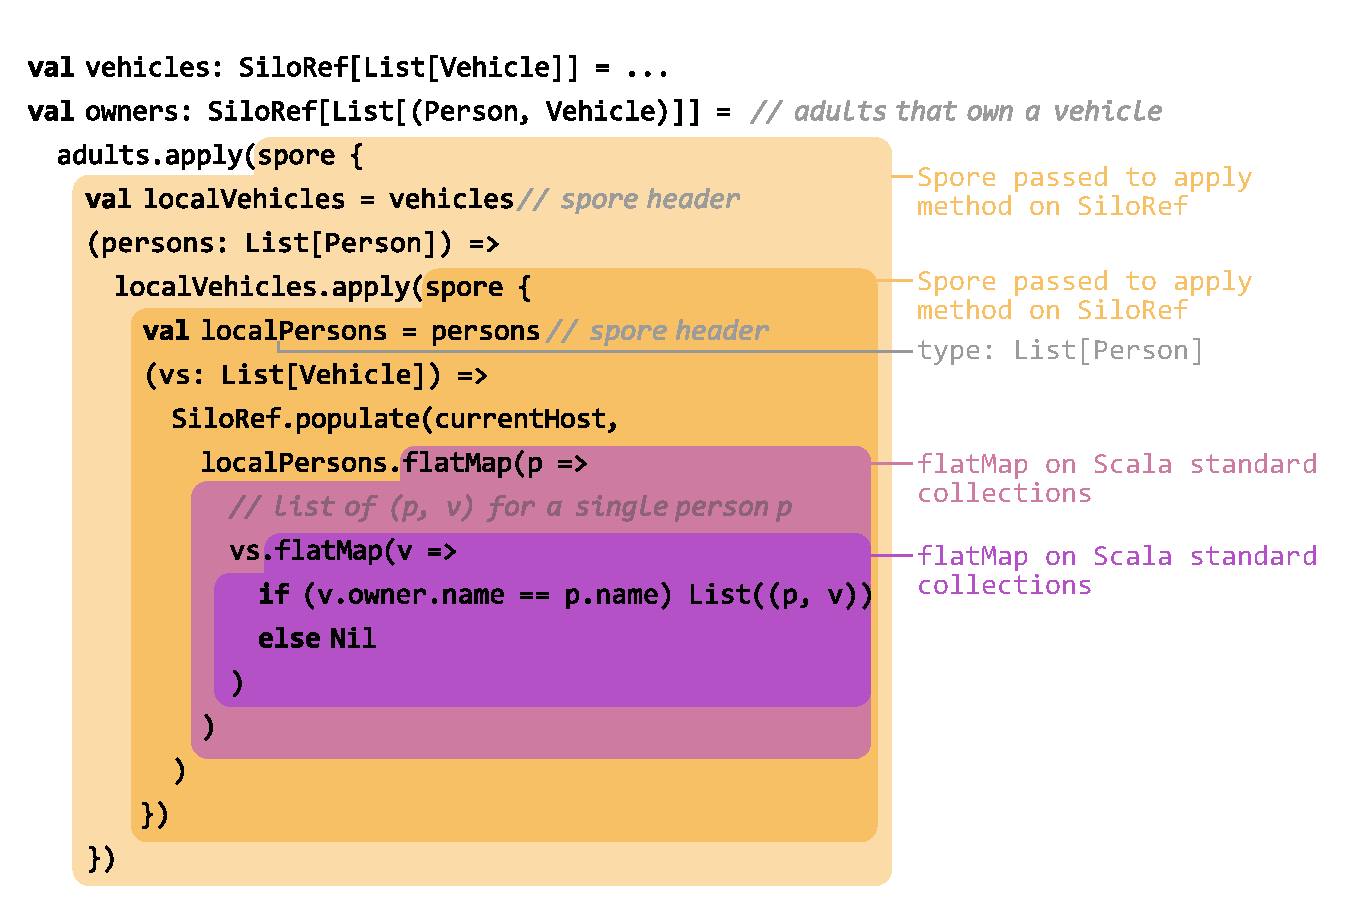
\includegraphics[scale=0.46]{diagram-annotated.pdf}
\caption{Matching persons and vehicle owners using the \texttt{apply} combinator.}\label{fig:apply-illustrated}
\end{figure}

\subsection{K-Means Clustering}\label{app:kmeans-illustrated}

Figure~\ref{fig:kmeans-illustrated} shows an illustrated version of
the listing of the k-means clustering example in
Section~\ref{sec:mbrace}.

\begin{figure}[ht!]
\centering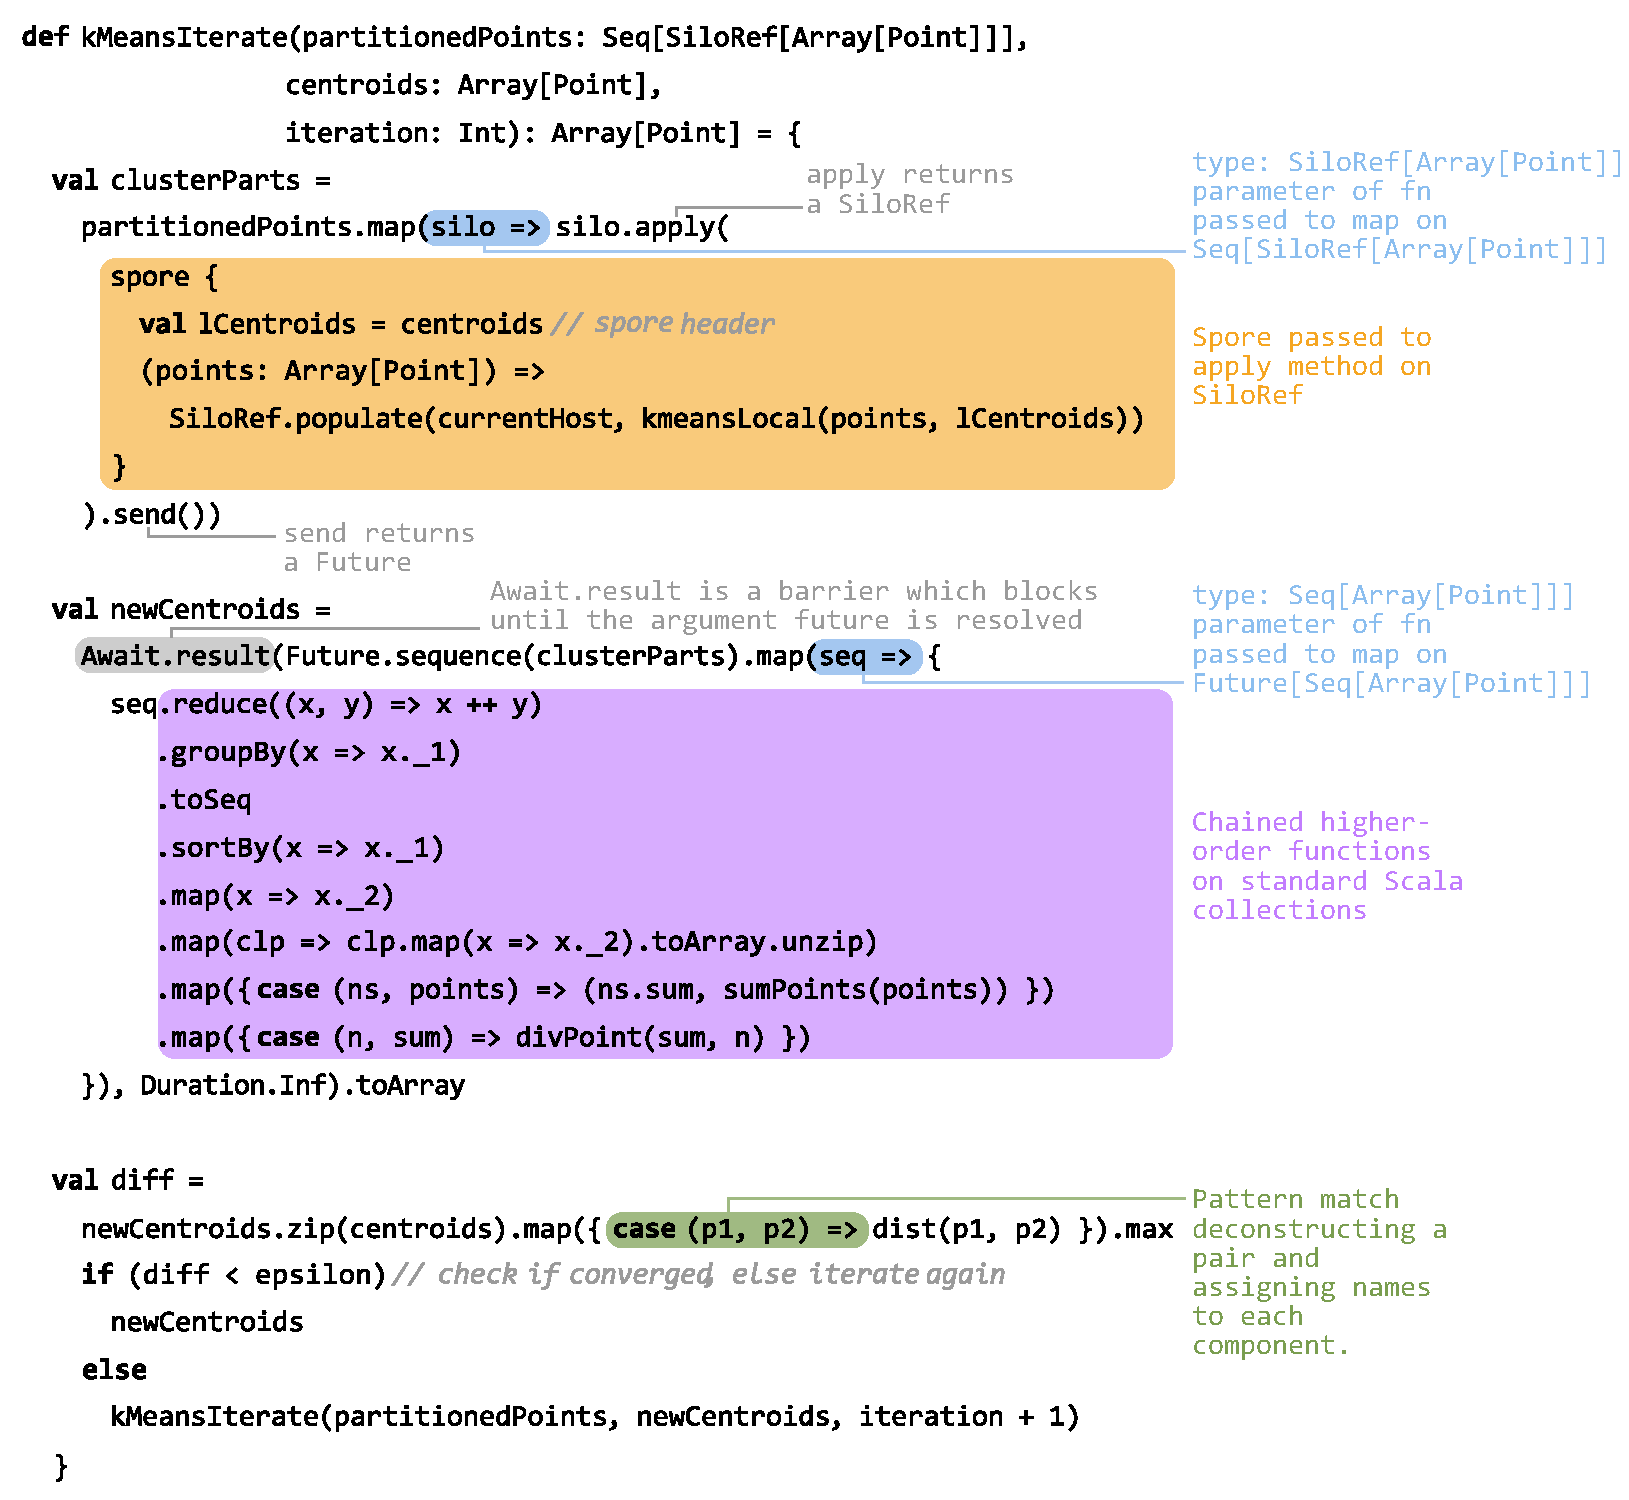
\includegraphics[scale=0.46]{k-means-annotated.pdf}
\caption{Excerpt of an implementation of k-means
  clustering.}\label{fig:kmeans-illustrated}
\end{figure}

\newpage
\section{Proofs}

\subsection{Proof of Theorem~\ref{lem:ser-values}}\label{app:ser-values}

\begin{thmun}
\emph{(Serializable Values)}
If $\Gamma ; \Sigma \vdash v : T$ and $serializable(T)$ then $\emptyset ; \Sigma \vdash v : T$.
\end{thmun}
\begin{proof}
By induction on the derivation of $\Gamma ; \Sigma \vdash v : T$ with a case analysis of the last applied rule.

\begin{itemize}
\item Cases \textsc{T-Int}, \textsc{T-Unit}, and \textsc{T-Host} are trivial.

\item Case \textsc{T-SiloRef}.
\begin{enumerate}
% 1.
\item By the assumptions
  \begin{enumerate}[label=(\alph*)]
  \item $\Gamma ; \Sigma \vdash v : T$
  \item $serializable(T)$
  \end{enumerate}
% 2.
\item By 1.a) and \textsc{T-SiloRef}
  \begin{enumerate}[label=(\alph*)]
  \item $v = {\Ref l h}$
  \item $T = \SR{T'}$
  \item $\Sigma(id(l)) = T'$
  \item $\Sigma \vdash {\Ref l h}$
  \end{enumerate}
% 3.
\item By 2.a-d), and \textsc{T-SiloRef}, $\emptyset ; \Sigma \vdash v : T$.
\end{enumerate}

\item Case \textsc{T-Spore} follows by \textsc{S-Spore} and the IH.
\end{itemize}
\end{proof}


\subsection{Proof of Theorem~\ref{th:subject-reduction}}\label{app:subject-reduction}

\begin{lem}
\emph{(Weakening)}\label{lem:weakening}
If $\Gamma ; \Sigma \vdash t : T$ and $x \notin dom(\Gamma)$, then
$\Gamma , x : T' ; \Sigma \vdash t : T$.
\end{lem}
\begin{proof}
By induction on the derivation of $\Gamma ; \Sigma \vdash t : T$.
\end{proof}

\begin{lem}
\emph{(Weakening of Store Typing)}\label{lem:weakening-store-typing}
\begin{enumerate}
\item If $\Gamma ; \Sigma \vdash t : T$ and $\iota \notin \mathit{dom}(\Sigma)$ then $\Gamma ; \Sigma' \vdash t : T$ where $\Sigma' = [\iota \mapsto T']\Sigma$.
\item If $\Sigma \vdash (t, \sigma)^h$ and $\iota \notin \mathit{dom}(\Sigma)$ then $\Sigma' \vdash (t, \sigma)^h$ where $\Sigma' = [\iota \mapsto T]\Sigma$.
\item If $\Sigma \vdash H$ and $\iota \notin \mathit{dom}(\Sigma)$ then $\Sigma' \vdash H$ where $\Sigma' = [\iota \mapsto T]\Sigma$.
\end{enumerate}
\end{lem}
\begin{proof}
Part 1: By induction on the derivation of $\Gamma ; \Sigma \vdash t : T$. Part 2: By induction on the derivation of $\Sigma \vdash (t, \sigma)^h$. Part 3: By induction on the derivation of $\Sigma \vdash H$.
\end{proof}

\begin{lem}\emph{(Process)}\label{lem:process}
If $\Sigma \vdash \sigma$, $\Sigma \vdash m$, and $process(h, m, \sigma) = (t, M, \sigma')$ then $\emptyset ; \Sigma' \vdash t : T$ for some $T$, $\Sigma' \vdash M$, and $\Sigma' \vdash \sigma'$ for some $\Sigma' \supseteq \Sigma$.
\end{lem}
\begin{proof}
\begin{itemize}
\item Case \textsc{Proc-Req}.
\begin{enumerate}
% 1.
\item By the assumptions
  \begin{enumerate}[label=(\alph*)]
  \item $\Sigma \vdash \sigma$
  \item $\Sigma \vdash m$
  \item $process(h, m, \sigma) = (t, M, \sigma')$
  \end{enumerate}
% 2.
\item By \textsc{Proc-Req}
  \begin{enumerate}[label=(\alph*)]
  \item $m = {\Req {h'} r \iota}$
  \item $r = {\Ref l h}$
  \item $\sigma(id(l)) = (v, P)$
  \item $M = \{ h' \leftarrow {\Res \iota v} \}$
  \item $\sigma' = {\consume {id(l)} P \sigma}$
  \item $t = \texttt{unit}$
  \end{enumerate}
% 3.
\item Define $\Sigma' := \Sigma$.
% 4.
\item By 2.e) and Def.~\ref{def:consume}, $dom(\sigma') \subseteq dom(\sigma)$.
% 5.
\item By 1.a), 3., 4., and \textsc{WF-Store1-3}, $\Sigma' \vdash \sigma'$.
% 6.
\item By 1.b), 2.a,b), and \textsc{WF-Req}
  \begin{enumerate}[label=(\alph*)]
  \item $\Sigma(id(l)) = \Sigma(\iota)$
  \item $\Sigma \vdash r$
  \end{enumerate}
% 7.
\item Define $T := \Sigma(id(l))$.
% 8.
\item By 1.a), 2.c), 7., and \textsc{WF-Store2}, $\emptyset ; \Sigma \vdash v : T$.
% 9.
\item By 6.a), 7., 8., and \textsc{WF-Res}, $\Sigma \vdash {\Res \iota v}$.
% 10.
\item By 2.d), 9., and \textsc{WF-Messages}, $\Sigma \vdash M$.
% 11.
\item By 2.f), \textsc{T-Unit}, and Lemma~\ref{lem:weakening-store-typing}, $\emptyset ; \Sigma \vdash t : T'$ for some $T'$.
% 12.
\item 3., 5., 10., and 11. close this case.
\end{enumerate}

\item Cases \textsc{Proc-ReqMat1}, \textsc{Proc-ReqMat2}, and \textsc{Proc-ReqParent} follow analogously.

\item Case \textsc{Proc-ReqApply}.
\begin{enumerate}
% 1.
\item By the assumptions
  \begin{enumerate}[label=(\alph*)]
  \item $\Sigma \vdash \sigma$
  \item $\Sigma \vdash m$
  \item $process(h, m, \sigma) = (t, M, \sigma')$
  \end{enumerate}
% 2.
\item By \textsc{Proc-ReqApply}
  \begin{enumerate}[label=(\alph*)]
  \item $m = {\Req {h'} r \iota}$
  \item $r = {\Ref l h}$
  \item $l = {\FMapped {\iota'} {l'} p}$
  \item $\sigma(id(l')) = (v, P)$
  \item $t = \texttt{respond}(h', \iota, \texttt{await}(\texttt{send}(p~v)))$
  \item $\sigma' = {\consume {id(l')} P \sigma}$
  \item $M = \emptyset$
  \end{enumerate}
% 3.
\item By 1.b), 2.a,b), and \textsc{WF-Req}
  \begin{enumerate}[label=(\alph*)]
  \item $\Sigma(id(l)) = \Sigma(\iota)$
  \item $\Sigma \vdash r$
  \end{enumerate}
% 4.
\item By 2.b,c), 3.b), \textsc{WF-Ref}, and \textsc{WF-Lin2}
  \begin{enumerate}[label=(\alph*)]
  \item $\Sigma(\iota') = T$
  \item $\Sigma(id(l')) = T'$
  \item $\exists \Gamma.~\Gamma ; \Sigma \vdash p : T' \Rightarrow \texttt{SiloRef}[T]~\{\ldots\}$
  \item $\Sigma \vdash l'$
  \end{enumerate}
% 5.
\item By 1.a), 2.d), 4.b), and \textsc{WF-Store2}, $\emptyset ; \Sigma \vdash v : T'$.
% 6.
\item By 4.c), \textsc{T-Spore}, Def.~$serializable$, and Lemma~\ref{lem:ser-values}, $\emptyset ; \Sigma \vdash p : T' \Rightarrow \texttt{SiloRef}[T]~\{\ldots\}$.
% 7.
\item By 5., 6., and \textsc{T-AppSpore}, $\emptyset, \Sigma \vdash p~v : \texttt{SiloRef}[T]$.
% 8.
\item By 7. and \textsc{T-Send}, $\emptyset, \Sigma \vdash \texttt{send}(p~v) : \texttt{Future}[T]$.
% 9.
\item By 8. and \textsc{T-Await}, $\emptyset, \Sigma \vdash \texttt{await}(\texttt{send}(p~v)) : T$.
% 10.
\item By 3.a), 4.a), and Def.~\ref{def:id}, $\Sigma(\iota) = T$ and thus by \textsc{T-Ident}, $\emptyset ; \Sigma \vdash \iota : \texttt{Future}[T]$.
% 11.
\item By 2.e), 9., 10., and \textsc{T-Respond}, $\emptyset, \Sigma \vdash t : \texttt{Unit}$.
% 12.
\item By 2.g) and \textsc{WF-Messages-Emp}, $\Sigma \vdash M$.
% 13.
\item By 2.f) and Def.~\ref{def:consume}, $dom(\sigma') \subseteq dom(\sigma)$.
% 14.
\item By 1.a), 13., and \textsc{WF-Store1-3}, $\Sigma \vdash \sigma'$.
% 15.
\item 11., 12., and 14. close this case.
\end{enumerate}

% TODO: expand for debugging
\item Cases \textsc{Proc-ReqPersist} and \textsc{Proc-Res} follow analogously.

\end{itemize}
\end{proof}


\begin{thmun}
\emph{(Subject Reduction)}

\begin{enumerate}

\item If $\Gamma ; \Sigma \vdash t : T$, $\Sigma \vdash \sigma$, and $t~|~\sigma \rightarrow^h t'~|~\sigma'$ then $\Gamma ; \Sigma' \vdash t' : T$ and $\Sigma' \vdash \sigma'$ for some $\Sigma' \supseteq \Sigma$.

\item If $\Sigma \vdash H~|~M$ and $H~|~M \twoheadrightarrow H'~|~M'$ then $\Sigma' \vdash H'~|~M'$ for some $\Sigma' \supseteq \Sigma$.

\end{enumerate}

\end{thmun}
\begin{proof}

Part 1: by induction on the derivation of $t~|~\sigma \rightarrow^h t'~|~\sigma'$ with case analysis of the last applied rule.

\begin{itemize}
\item Case \textsc{R-AppAbs}.
\begin{enumerate}
% 1.
\item By the assumptions
  \begin{enumerate}[label=(\alph*)]
  \item $\Gamma ; \Sigma \vdash t : T$
  \item $\Sigma \vdash \sigma$
  \item $t~|~\sigma \rightarrow^h t'~|~\sigma'$
  \end{enumerate}
% 2.
\item By \textsc{R-AppAbs}
  \begin{enumerate}[label=(\alph*)]
  \item $t = E[((x : T') \Rightarrow t'')~v']$
  \item $t' = E[[x \mapsto v']t'']$
  \item $\sigma' = \sigma$
  \end{enumerate}
% 3.
\item By 1.a) and 2.a), $\Gamma ; \Sigma \vdash ((x : T') \Rightarrow t'')~v' : T''$.
% 4.
\item By 3. and \textsc{T-App},
  \begin{enumerate}[label=(\alph*)]
  \item $\Gamma ; \Sigma \vdash ((x : T') \Rightarrow t'') : T' \Rightarrow T''$
  \item $\Gamma ; \Sigma \vdash v' : T'$
  \end{enumerate}
% 5.
\item By 4.a) and \textsc{T-Abs}, $\Gamma , x : T' ; \Sigma \vdash t'' : T''$.
% 6.
\item By 4.b), 5., and Lemma~\ref{th:subst}, $\Gamma ; \Sigma \vdash [x \mapsto v']t'' : T''$.
% 7.
\item By 1.a), 2.a-b), 3., and 6., $\Gamma ; \Sigma \vdash t' : T$.
% 8.
\item 2.c) and 7. close this case.
\end{enumerate}

\item Cases \textsc{R-IntOp}, \textsc{R-AppSpore}, and \textsc{R-Await} follow analogously.

\item Case \textsc{R-Apply}.
\begin{enumerate}
% 1.
\item By the assumptions
  \begin{enumerate}[label=(\alph*)]
  \item $\Gamma ; \Sigma \vdash t : T$
  \item $\Sigma \vdash \sigma$
  \item $t~|~\sigma \rightarrow^h t'~|~\sigma'$
  \end{enumerate}
% 2.
\item By \textsc{R-Apply}
  \begin{enumerate}[label=(\alph*)]
  \item $t  = E[\texttt{apply}(r, p)]$
  \item $r  = {\Ref l {h'}}$
  \item $t' = E[r']$
  \item $r' = {\Ref {l'} {h'}}$
  \item $l' = {\FMapped {(h, i)} l p}$ where $i~\text{fresh}$
  \item $\sigma' = \sigma$
  \end{enumerate}
% 3.
\item By 1.a) and 2.a), $\Gamma ; \Sigma \vdash \texttt{apply}(r, p) : \hat{T}$.
% 4.
\item By 3. and \textsc{T-Apply},
  \begin{enumerate}[label=(\alph*)]
  \item $\hat{T} = \texttt{SiloRef}[T']$
  \item $\Gamma ; \Sigma \vdash r : \texttt{SiloRef}[T'']$
  \item $\Gamma ; \Sigma \vdash p : T'' \Rightarrow \texttt{SiloRef}[T']~\{~\texttt{type}~\mathcal{C} = \seq{T}~\}$
  \end{enumerate}
% 5.
\item By 2.b), 4.b), \textsc{T-SiloRef}, and \textsc{WF-Ref}
  \begin{enumerate}[label=(\alph*)]
  \item $\Sigma(id(l)) = T''$
  \item $\Sigma \vdash r$
  \item $\Sigma \vdash l$
  \item $h' \in \mathcal{H}$
  \end{enumerate}
% 6.
\item Define $\Sigma' := [(h, i) \mapsto T']\Sigma$.
% 7.
\item By 2.d-e), 4.c), 5.a-d), 6., \textsc{WF-Lin2}, and \textsc{WF-Ref}, $\Sigma' \vdash r'$.
% 8.
\item By 2.d-e), 6., 7., and \textsc{T-SiloRef}, $\Gamma ; \Sigma' \vdash r' : \texttt{SiloRef}[T']$.
% 9.
\item By 2.e), 3., 4.a), 6., and part 1 of Lemma~\ref{lem:weakening-store-typing}, $\Gamma ; \Sigma' \vdash \texttt{apply}(r, p) : \texttt{SiloRef}[T']$.
% 10.
\item By 1.a), 2.e), 6., and part 1 of Lemma~\ref{lem:weakening-store-typing}, $\Gamma ; \Sigma' \vdash t : T$.
% 11.
\item By 2.a,c), 8., 9., and 10., $\Gamma ; \Sigma' \vdash t' : T$.
% 12.
\item By 1.b) and 2.f), $\Sigma \vdash \sigma'$.
% 13.
\item By 6., $\Sigma' \supseteq \Sigma$.
% 14.
\item By 12., 13., and \textsc{WF-Store3}, $\Sigma' \vdash \sigma'$.
% 15.
\item 11., 13., and 14. close this case.

\end{enumerate}

\item Cases \textsc{R-Persist} and \textsc{R-Unpersist} follow analogously.
\end{itemize}

%
Part 2: by induction on the derivation of $H~|~M \twoheadrightarrow H'~|~M'$ with case analysis of the last applied rule.

\begin{itemize}
\item Case \textsc{R-Local}.
\begin{enumerate}
% 1.
\item By the assumptions
  \begin{enumerate}[label=(\alph*)]
  \item $\Sigma \vdash H~|~M$
  \item $H~|~M \twoheadrightarrow H'~|~M'$
  \end{enumerate}
% 2.
\item By \textsc{R-Local}
  \begin{enumerate}[label=(\alph*)]
  \item $H = \{ (t, \sigma)^h \} \cup H''$
  \item $H' = \{ (t', \sigma')^h \} \cup H''$
  \item $t~|~\sigma \rightarrow^h t'~|~\sigma'$
  \item $M' = M$
  \end{enumerate}
% 3.
\item By 1.a) and \textsc{WF-Config}, $\Sigma \vdash H$.
% 4.
\item By 2.a), 3., and \textsc{WF-Host2}
  \begin{enumerate}[label=(\alph*)]
  \item $\Sigma \vdash (t, \sigma)^h$
  \item $\Sigma \vdash H''$
  \end{enumerate}
% 5.
\item By 4.a) and \textsc{WF-HostConfig}
  \begin{enumerate}[label=(\alph*)]
  \item $\Sigma \vdash \sigma$
  \item $\Gamma ; \Sigma \vdash t : T$ for some $\Gamma$
  \end{enumerate}
% 6.
\item By 2.c), 5.a,b), and part 1
  \begin{enumerate}[label=(\alph*)]
  \item $\Gamma ; \Sigma' \vdash t' : T$
  \item $\Sigma' \vdash \sigma'$ for some $\Sigma' \supseteq \Sigma$
  \end{enumerate}
% 7.
\item By 6.a,b) and \textsc{WF-HostConfig}, $\Sigma' \vdash (t', \sigma')^h$.
% 8.
\item By 4.b), 6.b), and part 3 of Lemma~\ref{lem:weakening-store-typing}, $\Sigma' \vdash H''$.
% 9.
\item By 2.b), 7., 8., and \textsc{WF-Host2}, $\Sigma' \vdash H'$.
% 10.
\item By 1.a), 2.d), 9., \textsc{WF-Config}, and \textsc{WF-Messages}, $\Sigma' \vdash H'~|~M'$.
\end{enumerate}

\item Case \textsc{R-Send}.
\begin{enumerate}
% 1.
\item By the assumptions
  \begin{enumerate}[label=(\alph*)]
  \item $\Sigma \vdash H~|~M$
  \item $H~|~M \twoheadrightarrow H'~|~M'$
  \end{enumerate}
% 2.
\item By \textsc{R-Send}
  \begin{enumerate}[label=(\alph*)]
  \item $H  = \{ (E[\texttt{send}(r)], \sigma)^h \} \cup H''$
  \item $H' = \{ (E[id(l)], \sigma)^h \} \cup H''$
  \item $r  = {\Ref l {h'}}$
  \item $m  = {\Req h r {id(l)}}$
  \item $M' = M \uplus \{ h' \leftarrow m \}$
  \end{enumerate}
% 3.
\item By 1.a) and \textsc{WF-Config}
  \begin{enumerate}[label=(\alph*)]
  \item $\Sigma \vdash H$
  \item $\Sigma \vdash M$
  \end{enumerate}
% 4.
\item By 2.a), 3.a), and \textsc{WF-Host2}
  \begin{enumerate}[label=(\alph*)]
  \item $\Sigma \vdash (E[\texttt{send}(r)], \sigma)^h$
  \item $\Sigma \vdash H''$
  \end{enumerate}
% 5.
\item By 4.a) and \textsc{WF-HostConfig}
  \begin{enumerate}[label=(\alph*)]
  \item $\Sigma \vdash \sigma$
  \item $\Gamma ; \Sigma \vdash E[\texttt{send}(r)] : T$ for some $\Gamma$
  \end{enumerate}
% 6.
\item By 5.b), $\Gamma ; \Sigma \vdash \texttt{send}(r) : \hat{T}$.
% 7.
\item By 6. and \textsc{T-Send}
  \begin{enumerate}[label=(\alph*)]
  \item $\hat{T} = \texttt{Future}[T'']$
  \item $\Gamma ; \Sigma \vdash r : \texttt{SiloRef}[T'']$
  \end{enumerate}
% 8.
\item By 2.c), 7.b), and \textsc{T-SiloRef}
  \begin{enumerate}[label=(\alph*)]
  \item $\Sigma(id(l)) = T''$
  \item $\Sigma \vdash r$
  \end{enumerate}
% 9.
\item By 8.a) and \textsc{T-Ident}, $\Gamma ; \Sigma \vdash id(l) : \texttt{Future}[T'']$.
% 10.
\item By 5.b), 6., 7.a), and 9., $\Gamma ; \Sigma \vdash E[id(l)] : T$.
% 11.
\item By 5.a), 10., and \textsc{WF-HostConfig}, $\Sigma \vdash (E[id(l)], \sigma)^h$.
% 12.
\item By 4.b), 11., and \textsc{WF-Host2}, $\Sigma \vdash H'$.
% 13.
\item By 2.c,d), 8.b), and \textsc{WF-Req}, $\Sigma \vdash m$.
% 14.
\item By 2.c,e), 3.b), 8.b), 13., \textsc{WF-Ref}, and \textsc{WF-Messages}, $\Sigma \vdash M'$.
% 15.
\item By 12., 14., and \textsc{WF-Config}, $\Sigma \vdash H'~|~M'$.
\end{enumerate}

\item Cases \textsc{R-Populate} and \textsc{R-Respond} follow analogously.

\item Case \textsc{R-Process}.
\begin{enumerate}
% 1.
\item By the assumptions
  \begin{enumerate}[label=(\alph*)]
  \item $\Sigma \vdash H~|~M$
  \item $H~|~M \twoheadrightarrow H'~|~M'$
  \end{enumerate}
% 2.
\item By \textsc{R-Process}
  \begin{enumerate}[label=(\alph*)]
  \item $H  = \{ (E[\texttt{await}(\iota)], \sigma)^h \} \cup H''$
  \item $H' = \{ (E[t~;~\texttt{await}(\iota)], \sigma')^h \} \cup H''$
  \item $M' = \hat{M} \uplus M''$
  \item $process(h, m, \sigma) = (t, M'', \sigma')$
  \item $M = \hat{M} \uplus \{ h \leftarrow m \}$
  \end{enumerate}
% 3.
\item By 1.a) and \textsc{WF-Config}
  \begin{enumerate}[label=(\alph*)]
  \item $\Sigma \vdash H$
  \item $\Sigma \vdash M$
  \end{enumerate}
% 4.
\item By 2.a), 3.a), and \textsc{WF-Host2}
  \begin{enumerate}[label=(\alph*)]
  \item $\Sigma \vdash (E[\texttt{await}(\iota)], \sigma)^h$
  \item $\Sigma \vdash H''$
  \end{enumerate}
% 5.
\item By 4.a) and \textsc{WF-HostConfig}
  \begin{enumerate}[label=(\alph*)]
  \item $\Sigma \vdash \sigma$
  \item $\Gamma ; \Sigma \vdash E[\texttt{await}(\iota)] : T$ for some $\Gamma$
  \end{enumerate}
% 6.
\item By 2.e), 3.b), and \textsc{WF-Messages}, $\Sigma \vdash m$.
% 7.
\item By 2.d), 5.a), 6., and Lemma~\ref{lem:process}~(Process), $\exists \Sigma', T'$ such that
  \begin{enumerate}[label=(\alph*)]
  \item $\emptyset ; \Sigma' \vdash t : T'$
  \item $\Sigma' \vdash M''$
  \item $\Sigma' \vdash \sigma'$
  \item $\Sigma' \supseteq \Sigma$
  \end{enumerate}
% 8.
\item By 5.b), 7.d), and part 1 of Lemma~\ref{lem:weakening-store-typing}, $\Gamma ; \Sigma' \vdash E[\texttt{await}(\iota)] : T$.
% 9. XXX
\item By 7.a) and 8., $\Gamma ; \Sigma' \vdash E[t~;~\texttt{await}(\iota)] : T$.
% 10.
\item By 7.c), 9., and \textsc{WF-HostConfig}, $\Sigma' \vdash (E[t~;~\texttt{await}(\iota)], \sigma')^h$.
% 11.
\item By 4.b), 7.d), and part 3 of Lemma~\ref{lem:weakening-store-typing}, $\Sigma' \vdash H''$.
% 12.
\item By 2.b), 10., 11., and \textsc{WF-Host2}, $\Sigma' \vdash H'$.
% 13.
\item By 3.b), 7.d), \textsc{WF-Res}, \textsc{WF-Req}, \textsc{WF-Ref}, and \textsc{WF-Messages}, $\Sigma' \vdash M$.
% 14.
\item By 2.c), 2.e), 7.b), 13., and \textsc{WF-Messages}, $\Sigma' \vdash M'$.
% 15.
\item By 12., 14., and \textsc{WF-Config}, $\Sigma' \vdash H'~|~M'$.
\end{enumerate}

\item Case \textsc{R-Process-Val}.
\begin{enumerate}
% 1.
\item By the assumptions
  \begin{enumerate}[label=(\alph*)]
  \item $\Sigma \vdash H~|~M$
  \item $H~|~M \twoheadrightarrow H'~|~M'$
  \end{enumerate}
% 2.
\item By \textsc{R-Process-Val}
  \begin{enumerate}[label=(\alph*)]
  \item $H  = \{ (v, \sigma)^h \} \cup H''$
  \item $H' = \{ (t, \sigma')^h \} \cup H''$
  \item $M' = \hat{M} \uplus M''$
  \item $process(h, m, \sigma) = (t, M'', \sigma')$
  \item $M = \hat{M} \uplus \{ h \leftarrow m \}$
  \end{enumerate}
% 3.
\item By 1.a) and \textsc{WF-Config}
  \begin{enumerate}[label=(\alph*)]
  \item $\Sigma \vdash H$
  \item $\Sigma \vdash M$
  \end{enumerate}
% 4.
\item By 2.a), 3.a), and \textsc{WF-Host2}
  \begin{enumerate}[label=(\alph*)]
  \item $\Sigma \vdash (v, \sigma)^h$
  \item $\Sigma \vdash H''$
  \end{enumerate}
% 5.
\item By 4.a) and \textsc{WF-HostConfig}
  \begin{enumerate}[label=(\alph*)]
  \item $\Sigma \vdash \sigma$
  \item $\Gamma ; \Sigma \vdash v : T$ for some $\Gamma$
  \end{enumerate}
% 6.
\item By 2.e), 3.b), and \textsc{WF-Messages}, $\Sigma \vdash m$.
% 7.
\item By 2.d), 5.a), 6., and Lemma~\ref{lem:process}~(Process), $\exists \Sigma', T'$ such that
  \begin{enumerate}[label=(\alph*)]
  \item $\emptyset ; \Sigma' \vdash t : T'$
  \item $\Sigma' \vdash M''$
  \item $\Sigma' \vdash \sigma'$
  \item $\Sigma' \supseteq \Sigma$
  \end{enumerate}
% 8.
\item By 7.a), 7.c), and \textsc{WF-HostConfig}, $\Sigma' \vdash (t, \sigma')^h$.
% 9.
\item By 4.b), 7.d), and part 3 of Lemma~\ref{lem:weakening-store-typing}, $\Sigma' \vdash H''$.
% 10.
\item By 2.b), 8., 9., and \textsc{WF-Host2}, $\Sigma' \vdash H'$.
% 11.
\item By 3.b), 7.d), \textsc{WF-Res}, \textsc{WF-Req}, \textsc{WF-Ref}, and \textsc{WF-Messages}, $\Sigma' \vdash M$.
% 12.
\item By 2.c), 2.e), 7.b), 11., and \textsc{WF-Messages}, $\Sigma' \vdash M'$.
% 13.
\item By 10., 12., and \textsc{WF-Config}, $\Sigma' \vdash H'~|~M'$.
\end{enumerate}

\end{itemize}

\end{proof}

\subsection{Proof of Theorem~\ref{thm:finite-mat}}\label{app:finite-mat}

\begin{lem}[Responsive Population]\label{lem:resp-population}
  Let $\Sigma \vdash H~|~M~|~R$ and $H = \{ (E[t], \sigma)^h \} \uplus
  \hat{H}$.

  Then $\forall h' \in \mathit{hosts}(H)$: $\{ (E[\texttt{send}(r)],
  \sigma)^h \} \uplus \hat{H}~|~M \uplus \{ h' \leftarrow m \}
  \twoheadrightarrow^* H'~|~M' \uplus \{ h \leftarrow m \}$ after a
  finite number of reduction steps where $r = {\Ref l {h'}}$, $l =
  {\Mat \iota}$ for some $\iota$, and $m = {\Res \iota v}$.
\end{lem}
\begin{proof}[Proof Sketch]
  By \textsc{R-Send}, $\{ (E[\texttt{send}(r)], \sigma)^h \} \uplus
  \hat{H}~|~M \uplus \{ h' \leftarrow m \} \twoheadrightarrow \{
  (E[\iota], \sigma)^h \} \uplus \hat{H}~|~M \uplus \{ h' \leftarrow m
  \} \uplus \{ h' \leftarrow m' \}$ where $m' = {\Req h r \iota}$.
  By Def.~\ref{def:fair-scheduling} message $m$ is processed by $h'$
  after a finite number of reduction steps. As a result, the store of
  $h'$ is updated with the mapping $\iota \mapsto v$. After another
  finite number of reduction steps, $h'$ processes message $m'$. By
  \textsc{R-Process}, \textsc{R-Process-Val}, and
  \textsc{Proc-ReqMat1}, the resulting multiset of messages includes
  $\{h \leftarrow {\Res \iota v} \}$ as required.
\end{proof}

\begin{lem}[Responsive Apply]\label{lem:resp-apply}
\end{lem}
\begin{proof}
\begin{enumerate}
  % 1.
\item By \textsc{R-Local} and \textsc{R-Apply}
  \begin{enumerate}[label=(\alph*)]
  \item $E[\texttt{apply}(r, p)]~|~\sigma \rightarrow^h E[r']~|~\sigma~|~\{ r' \}$
  \item $r' = {\Ref {l'} {h'}}$
  \item $r = {\Ref l {h'}}$
  \item $l' = {\FMapped {(h, i)} l p}$ where $i$ fresh
  \item $H' = \{ (E[r'], \sigma)^h \} \uplus \hat{H}$
  \item $M' = M$
  \item $R' = R \uplus \{ r' \}$
  \end{enumerate}
  % 2.
\item By Lemma~\ref{lem:resp}, $\mathit{Responsive}(H', M', R)$.
  % 3.
\item Consider $H'~|~M' \uplus \{h' \leftarrow m\}~|~R'$ where $m =
  {\Req {h''} {r'} \iota}$.
  % 4.
\item By Def.~\ref{def:fair-scheduling} $H'~|~M' \uplus \{h'
  \leftarrow m\}~|~R' \twoheadrightarrow^* H_p~|~M_p~|~R_p$ such that
  $(E_p[\texttt{await}(\iota_p)], \sigma_p)^{h'} \in H_p \lor
  (E_p[v_p], \sigma_p)^{h'} \in H_p$ and $\{h' \leftarrow m\} \in
  M_p$.
  % 5.
\item There are two cases. {\em Case 1:} $id(l) \notin
  \mathit{dom}(\sigma')$. In this case $H_p~|~M_p~|~R_p$ can be
  reduced according to \textsc{R-Process} (or \textsc{R-Process-Val})
  and \textsc{Proc-ReqParent}. As a result, $h'$ reduces
  $\texttt{send}({\Ref l {h'}})$. By \textsc{R-Send}, ${\Ref l {h'}}
  \in R$, and Lemma~\ref{lem:resp}, $H_p~|~M_p~|~R_p
  \twoheadrightarrow^* H_r~|~M_r \uplus \{h' \leftarrow {\Res {id(l)}
    v} \}~|~R_r$ after a finite number of reduction steps. By
  Def.~\ref{def:fair-scheduling} and \textsc{Proc-Res}, $H_r~|~M_r
  \uplus \{h' \leftarrow {\Res {id(l)} v} \}~|~R_r
  \twoheadrightarrow^* H''~|~M''~|~R''$ after a finite number of
  reduction steps, such that
  \begin{enumerate}[label=(\alph*)]
  \item $H'' = \{ (E'[t'], \sigma')^{h'} \} \cup H_3$ where $t' = v'$
    or $t' = \texttt{await}(\iota')$
  \item $M'' = \{h' \leftarrow m\} \uplus M_3$
  \item $\sigma'(id(l)) = v$
  \item $\Sigma'' \vdash H''~|~M''~|~R''$
  \end{enumerate}
  {\em Case 2:} $\sigma'(id(l)) = v$. In this case $H'' = H_p$, $M'' =
  M_p$, and $R'' = R_p$.
  % 6.
\item By 5.a-c), \textsc{R-Process}, \textsc{R-Process-Val}, and
  \textsc{Proc-ReqApply}
  \begin{enumerate}[label=(\alph*)]
  \item $\mathit{process}(h', m, \sigma') = (t'', \emptyset, \sigma')$
  \item $t'' = \texttt{respond}(h'', \iota, \texttt{await}(\texttt{send}(p~v)))$
  \item $H''~|~M''~|~R'' \twoheadrightarrow H_3~|~M_3~|~R''$
  \item $H_3 = \{ (E'[t''~\texttt{;}~t'], \sigma')^{h'} \} \cup H_4$
  \end{enumerate}
  % 7.
\item By 5.d), 6.c), and Theorem~\ref{th:subject-reduction} (Subject
  Reduction), $\Sigma_3 \vdash \{ (E'[t''~\texttt{;}~t'],
  \sigma')^{h'} \} \cup H_4~|~M_3~|~R''$ for some $\Sigma_3 \supseteq
  \Sigma''$.
  % 8.
\item By 7., \textsc{WF-Config}, \textsc{WF-Host2}, and \textsc{WF-HostConfig}
  \begin{enumerate}[label=(\alph*)]
  \item $\Sigma_3 \vdash \sigma'$
  \item $\Gamma_3 ; \Sigma_3 \vdash E'[t''~\texttt{;}~t'] : T_3$ for
    some $\Gamma_3$, $T_3$
  \end{enumerate}
  % 9.
\item By 6.b), 8.b), and the type rules
  \begin{enumerate}[label=(\alph*)]
  \item $\Gamma_4 ; \Sigma_3 \vdash p : T' \Rightarrow \texttt{SiloRef}[T]~\{~\texttt{type}~\mathcal{C} = \seq{T}~\}$ for some $\Gamma_4$
  \item $p = \texttt{spore}~\{~\seq{x : T = v}~; (x: T') \Rightarrow t~\}$
  \end{enumerate}
  % 10.
\item By 9.a,b), and \textsc{T-Spore}
  \begin{enumerate}[label=(\alph*)]
  \item $\seq{x : T}, x : T' ; \emptyset \vdash t : \texttt{SiloRef}[T]$
  \item $\forall S \in \seq{T}, \texttt{SiloRef}[T].~\mathit{serializable}(S)$
  \end{enumerate}
  % 11.
  \item By the type rules, derivation 10.a) does not contain
    applications of \textsc{T-SiloRef} or \textsc{T-Ident}. By 10.b)
    spore $p$ does not capture futures. Thus, any occurrence of
    $\texttt{await}(\hat{\iota})$ within $p~v$ is preceded by a
    reduction of a corresponding $\texttt{send}$ resulting in future
    $\hat{\iota}$. By Lemma~\ref{lem:resp} (Responsiveness),
    $\mathit{Responsive}(H_3, M_3, R)$. There are two cases.

    {\em Case 1:} $d = 0$. Then $p$ does not contain a nested
    \texttt{apply} invocation. Therefore, by
    Lemma~\ref{lem:resp-population}, $p~v$ reduces to a value $r''$
    after a finite number of reduction steps. Since either $r'' \in R$
    or $r''$ is newly populated, $\texttt{send}(r'')$ results in a
    response $h' \leftarrow {\Res {id(r'')} {v''}}$ after a finite
    number of reduction steps. This enables $h'$ to reduce
    $\texttt{respond}(h'', \iota, v'')$ which concludes this case.

    {\em Case 2:} $d > 0$. The depth of nested \texttt{apply}s of
    term $p~v$ is less than the depth of the term $\texttt{apply}(r,
    p)$.  Therefore, by the induction hypothesis, reductions of nested
    \texttt{apply} invocations within $p~v$ result in responsive
    configurations. By Lemma~\ref{lem:resp-population}, $p~v$ reduces
    to a value $r''$ after a finite number of reduction steps. Since
    either $r'' \in R$, or $r''$ is newly populated, or $r''$ is the
    result of a nested \texttt{apply} invocation,
    $\texttt{send}(r'')$ results in a response $h' \leftarrow {\Res
      {id(r'')} {v''}}$ after a finite number of reduction steps. This
    enables $h'$ to reduce $\texttt{respond}(h'', \iota, v'')$ which
    concludes this case.
\end{enumerate}
\end{proof}

\begin{thmun}
\emph{(Finite Materialization)}
  Let $\Sigma \vdash H~|~M~|~R$ such that $\mathit{Responsive}(H, M,
  R)$.

  If $H~|~M~|~R \twoheadrightarrow H'~|~M'~|~R'$ then
  $\mathit{Responsive}(H', M', R')$.
\end{thmun}
\begin{proof}
  Corollary of Lemma~\ref{lem:resp}, Lemma~\ref{lem:resp-population},
  and Lemma~\ref{lem:resp-apply}.
\end{proof}


\end{document}